\documentclass[12pt]{article}
\usepackage[utf8]{inputenc}
\usepackage{graphicx}

\usepackage{amssymb}
\usepackage{amsmath}
\usepackage{amsfonts}

% for tables
\usepackage{booktabs}
\usepackage{adjustbox}

% get a subsubsub section
\makeatletter
\renewcommand\paragraph{\@startsection{paragraph}{4}{\z@}%
            {-2.5ex\@plus -1ex \@minus -.25ex}%
            {1.25ex \@plus .25ex}%
            {\normalfont\normalsize\bfseries}}
\makeatother
\setcounter{secnumdepth}{4} % how many sectioning levels to assign numbers to
\setcounter{tocdepth}{4}    % how many sectioning levels to show in ToC

% for math
\usepackage{upgreek}

% for figures
\graphicspath{ {images/}
               {./../methods_figures}
               {./../results_figures} 
            }
% make bold -> "Figure 1.2:" ...
\usepackage[font=small, labelfont=bf]{caption}
% suppl. figures
\usepackage{newfloat}
\DeclareFloatingEnvironment[name={Supplementary Figure},fileext=lsf,listname={List of Supplementary Figures}]{suppfigure}
% referencing only figure number
% \usepackage{cleveref}
% place tables at specific locations
\usepackage{float}
\restylefloat{table}

% specify white space between list elements
\usepackage{enumitem}
\setlist{nosep}


\usepackage{caption}
\usepackage{subcaption}
\usepackage[a4paper,width=160mm,top=25mm,bottom=25mm,left=25mm,right=25mm]{geometry}
\usepackage{fancyhdr}
\pagestyle{fancy}
\fancyhead{}
\fancyhead[RO,LE]{Thesis Title}
\fancyfoot{}
\fancyfoot[LE,RO]{\thepage}
% \fancyfoot[LO,CE]{Chapter \thechapter}
% \fancyfoot[CO,RE]{Author Name}
\renewcommand{\headrulewidth}{0.4pt}
\renewcommand{\footrulewidth}{0.4pt}

\usepackage[style=authoryear,sorting=none,backend=bibtex]{biblatex}
\addbibresource{export.bib}

\title{Thesis Titless}
\author{Author Namesss}
\date{Day Month Yearss}

\begin{document}
\begin{titlepage}
    \begin{center}
        \vspace*{1cm}
        
        \Huge
        \textbf{Multiple axon tracking for biohybrid brain computer interfaces
        from directional living neural networks}
        
        \vspace{0.5cm}
        \LARGE
        Thesis Subtitle
        
        \vspace{1.5cm}
        
        \textbf{Author Name}
        
        \vfill
        
        A thesis presented for the degree of\\
        Doctor of Philosophy
        
        \vspace{0.8cm}
        
        \Large
        Department Name\\
        University Name\\
        Country\\
        Date
        
    \end{center}
\end{titlepage}
\clearpage

\thispagestyle{plain}
\begin{center}
    \section{Abstract}
    \vspace{0.4cm}
\end{center}
Lorem ipsum dolor sit amet, consectetur adipisicing elit, sed do eiusmod tempor incididunt ut labore et dolore magna aliqua. Ut enim ad minim veniam, quis nostrud exercitation ullamco laboris nisi ut aliquip ex ea commodo consequat. Duis aute irure dolor in reprehenderit in voluptate velit esse cillum dolore eu fugiat nulla pariatur. Excepteur sint occaecat cupidatat non proident, sunt in culpa qui officia deserunt mollit anim id est laborum.
Lorem ipsum dolor sit amet, consectetur adipisicing elit, sed do eiusmod tempor incididunt ut labore et dolore magna aliqua. Ut enim ad minim veniam, quis nostrud exercitation ullamco laboris nisi ut aliquip ex ea commodo consequat. Duis aute irure dolor in reprehenderit in voluptate velit esse cillum dolore eu fugiat nulla pariatur. Excepteur sint occaecat cupidatat non proident, sunt in culpa qui officia deserunt mollit anim id est laborum.
Lorem ipsum dolor sit amet, consectetur adipisicing elit, sed do eiusmod tempor incididunt ut labore et dolore magna aliqua. Ut enim ad minim veniam, quis nostrud exercitation ullamco laboris nisi ut aliquip ex ea commodo consequat. Duis aute irure dolor in reprehenderit in voluptate velit esse cillum dolore eu fugiat nulla pariatur. Excepteur sint occaecat cupidatat non proident, sunt in culpa qui officia deserunt mollit anim id est laborum.
\clearpage

\tableofcontents
\clearpage

\let\LaTeXStandardClearpage\clearpage
\let\clearpage\relax  % Do nothing when a \clearpage command appears 
\listoffigures
\listofsuppfigures
\let\clearpage\LaTeXStandardClearpage % Return to the old definition
\listoftables
\clearpage

\Large{\textbf{List of Abbriviations}} \\ \\

\normalsize
CLSM  -  Confocal laser scanning microscope
PDMS
CNN
MOTA

DI deionized
PDL
PBS phosphate buffered saline
CAD

CNS
DBS

MEA

dLGN

MOT

R-CNN

IQR inter quartile range

AAV

GFP
\clearpage

\section{Introduction}


Think of this as the funnel into your results story 
What does the reader need to know to understand the results. It should not feel 
like they come out of the blue. What's the context.

This can include: Which problem are you addressing? 

For which domains is the addressed problem relevant? 

Th intro should roughly map to the results order:
    model -> 20 structure screen -> (primitives)

It. can. be. short>:) \\

I hate this pseudo sophisticated research  jargon. I can't have that in my thesis. Please avoid it. \\


Broad scope approach-motivation statement \\
Funnel into short abstract-like summary of the project \\
background in three sections: biohybrid BCI, direcitonal networks, MOT \\
research problem, research aims + presented solution,  significance + which value \\


Why do we need directional neural networks?
    general entry funnel
    biohybrid interfaces
    disease models (sprinkle of bottom up neuroscience)

which efforts have been made to make networks directional?
    orient to csabas paper

Which solution does this work provide?
    primitives screen
    20 test structures screen






\newpage
\subsection{Outline}
Understanding the human brain requires neuroscience to develop complexity
reducing model systems that capture relevant functional, anatomical or chemical
features. The evaluation of which abstraction level and thus model system is
appropriate for answering key functional questions about the brain has long been
a source of controversy. This discussion is fundamentally rooted in the tension
between losing essential features in overly simplified model systems, and
dealing with overwhelming complexity and low experimental throughput in model
systems more closely resembling the human brain. \\
Although this work broadly employs \textit{in vitro} model systems thus trading
off resemblance to real brains for higher throughput and reduced complexity, it
is not primarily motivated by a certainty that this high abstraction level will
indeed \textit{solve} fundamental neuroscientific questions. Instead, this
project aims to follow an approach that has led to notable progress in other
domains, most prominently artificial intelligence: Developing an understanding
of the system by engineering it. This method has found adoption in domains as
neuromorphic engineering \parencite{neuromorphic} and neural engineering
\parencite{neuroengineering}, with the latter focusing i.a. on building
technology from living neural systems. Guided by the engineering problems, the
hope of these domains is that relevant neuroscientific questions are answered
along the way. And even if this does not come true, advancement in these fields
may still result in useful new technologies. The science presented here follows
this pursuit.\\ 

You can only do engineering at that scale. that's why were at that scale. DId
you make that clear enough? Inconsistency:  you mention this here in the
beginning but this idea is not really found thoughout the introduction.
Motivation is put on bad stimulation ability, and bad in vitro network models. 

In this work, \dots [abstract like but shorter]
f\\
f\\
f\\
f\\
f\\
f\\
f\\
f\\


\subsection{Biohybrid neural interfaces}
Neuroelectric interfacing based on metal electrodes has made remarkable progress
over the last decades (\cite{utaharray}, \cite{neuropixel}). These technologies
excel at locally confined high resolution neural recording for a time period on
the order of weeks. However, given the immense challenges related to high
quality neural interfacing \parencite{mooreslaw}, naturally, existing recording
and particularly stimulation technology exhibit shortcomings.
% # clearly say that stimulation works worse than recording
The clinically most adapted CNS stimulation method, deep brain stimulation
(DBS), does not specifically depolarize single neurons but instead exerts
various modulatory effects on entire brain areas \parencite{dbs}. Low
spatiotemporal resolution may be tolerable for common DBS applications, however,
addressing the clinically highly relevant cases of vision-, touch-, or hearing
loss is currently limited by insufficient resolution
\parencite{retinastimulation}. Another issue affecting both stimulation and
conventional neural recording systems is the induced foreign body response. Due
to natural brain movement, rigid metal electrodes cause inflammation, neuronal
cell death and glia formation while simultaneously, conventional electrode
insulation undergoes biodegradation resulting in decreased impedance
(\cite{eletrodeproblems1}, \cite{eletrodeproblems2}, \cite{eletrodeproblems3},
\cite{eletrodeproblems4}). In research applications, central nervous system
(CNS) stimulation is most commonly performed through optogenetic tools
(\cite{optog1}, \cite{optog2}). While the cell-type specificity of optogenetics
can be of great value, the limitations in spatial resolution inherent to in vivo
light-based technology seem to be a major hurdle for increasing spatial
resolution. On top of this, the risk of genetic off-target effects and adeno
associated virus (AAV) immune responses restrict medical use cases in the near
term \parencite{optogImmunresponse}. \\

Biohybrid implants take a fundamentally different approach to neural
interfacing, drawing inspiration from tissue engineering and in vitro
neuroscience. First described by \cite{biohybridfirst}, this promising
technology aims to solve the latent issue of biocompatibility by moving towards
the integration of biological components \parencite{biohybridreview}. At the
same time, biohybrid technology may benefit from the highly impressive
\textit{spec sheet} of a neuron, including energy efficiency, self-containment,
and signal transmission properties. Whilst engineering with neural tissue
presents almost daunting challenges, the biocompatibility prospects of biohybrid
interfaces are currently unaccessible by competing technologies. CNS
applications of the biohybrid approach include the coating of metal electrodes
with host cells (\cite{seededelectrodes1}, \cite{seededelectrodes2}), and the
use of ectopic axons as electrodes (\cite{filmbasedinterface},
\cite{cullenrecent}). The currently most advanced biohybrid implant is based on
a hydrogel microcolumn containing ectopic cortical axons that are optogentically
driven through an light emitting diode (LED) optical fiber outside the brain
\parencite{cullenrecent}. While synapse formation was shown anatomically in
vitro, the in vivo proof-of-concept implantation did not go as far as showing
functional target tissue innervation. \\

Current biohybrid implants trade off biocompatibility for interface bandwidth
and control. For example, the biohybrid implant presented in \cite{cullenrecent}
relied on optically exciting the entire ectopically grown neural population,
resulting in limited control of delivered stimulation. While this spatial
resolution may be sufficient for specific use cases, this implant design offers
insufficient control for delivering high dimensional data, such as sensory
input. For addressing the pressing issue of functionally restoring sensory
modalities \parencite{blindnesssux}, a biohybrid implant needs to allow for
stimulating independent channels. To solve this crucial design requirement, the
implant presented here is based on a PDMS micro fluidic system enabling the
independent stimulation of axons grown in micro channels. Briefly, PDMS
membranes are placed on coated glass dishes and seeded with RGC spheroids. Axons
extend through the 6 $\upmu$m high channel system until they reach the 3 mm long
output channel which will eventually be implanted. The final device will utilise
stretchable AuTiO\textsubscript{2} nanowire electrical contact pads for
stimulating RGC axons \parencite{nanowires}. Long term host cell survival will
be ensured by having the implant face the brain surface such that RGC spheroids
are integrated with the CNS microenvironment. The device will be implanted
targeting the dorsal lateral geniculate nucleus (dLGN). (illustration needed) 



\subsection{Engineered directional neural networks}
It is well established that the connectivity within biological neural networks
is a major determinant of the emerging electrophysiological dynamics. For
example, the microcircuit of the cat visual cortex exhibits a high degree of
sparsity with predominantly local inhibitory-, and excitatory connections to
achieve its output \parencite{ctxcircuit}. Despite the general agreement on the
significance of neural circuits, the vast majority of in vitro models remain
limited to random connectivity schemes. Neglecting this property of in vivo
neural networks may be well justified in studies that focus on basic biological
properties, for example in response to drug admission. However, any model system
investigating higher level functional properties emerging at the circuits-level
(e.g. learning mechanisms) requires confined connectivity. \\

More elaborately controlled connectivity schemes are indispensable for
technology relying on living neural circuits. Biohybrid interfaces as described
above rely fundamentally on directional connectivity. Innervation of neighboring
RGC source wells may result in activity dynamics independent of the imposed
electrical stimulation pattern, rendering single stimulation channels or the
entire device unusable. For this reason it is crucial for viable biohybrid
implants to achieve high degrees of growth directionality. \\
Likewise, more sophisticated models focusing on functional aspects of the
peripheral nervous system (PNS) may benefit from directional in vitro models.
PNS circuits generally show a pattern where sensory-, or motor axons converge to
form a nerve that eventually diverges again in the target location. Building an
in vitro platform resembling this architecture would be extremely useful for
studying neuropathy, traumatic nerve injury, tissue reinnervation and
[neurapraxia, axonotmesis, neurotmesis ?], and the effects of nerve stretching. 
The canonical design of the biohybrid implant where multiple RGC source nodes
converge into a common output channel replicates this motif. \\

% While pathological questions regarding the nerve itself may be investigated with
% artificial nerve models of limited directional connectivity
% \parencite{3dnervemodel}, functionally more complex pathologies, for example
% those related to development require directionally constraint in vitro models.
% \\

The challenge of achieving directional in vitro networks is often reduced to
imposing axonal or dendritic growth constraints once the neurons are seeded.
Although it is conceivable that initially randomly connected neural networks
develop directional connections solely by an electrically imposed activity
pattern \parencite{stdp}, this approach has so far been to no avail. Therefore,
various in vivo inspired approaches have been taken to instead induce control on
axonal outgrowth. Axon guidance mechanisms in vivo rely, broadly speaking, on
two categories of cues: mechanical and chemical ones (\cite{mechanicalcues},
\cite{chemicalcues}). Chemcial cues have been employed for guidance by
integrating substrate surface modifications favoring certain growth paths.
Although many attempts are limited to micro patterning with PDL falling short of
the highly complex chemical micro environment observed in vivo, still, a notable
degree of axonal growth control is achieved \parencite{singlecellmCP}. While
chemical guidance remains a promising direction for engineering defined neural
networks in the future, mechanical guidance has shown more promising results at
larger network scales \parencite{forro}. 

The idea of utilizing mechanical growth guidance in vitro is largely based on
advances in microfluidics for neuroscience (\cite{microfludics1},
\cite{microfludics2}).  These platforms are commonly fabricated from
Polydimethylsiloxane (PDMS), a polymer that can be molded at high resolution
using soft lithography, while also exhibiting acceptable biocompatibility
properties \parencite{pdms}. 3D mechanical guidance principles are based on the
inertia of growing axons, e.g. the inability to grow in sharp turns, and the
tendency of axons to attach to edges \parencite{axongrowth3d}. These two
findings are the basis of numerous PDMS design motifs proposed in the literature
to achieve directional growth through PDMS micro structures: barbed-, and
narrowing channels, (\cite{lefeber}, \cite{peyrin},) redirecting hooks and
consecutive arches (\cite{pirlo}, \cite{na}, \cite{renault},
\cite{2019afterForro}), and diode-like triangles (\cite{gladkov},
\cite{isomura}). So far, the most competitive multi node directional networks
are based on a relatively simple motif, where axons detachment from sharp radii
prevents growth in the undesired direction \parencite{forro}. \\

While \cite{forro} presented respectable results for four-node-networks, the
nerve model system and surely the biohybrid implant require an order of
magnitude more nodes, while also deviating from the rather simple one-to-one
connectivity scheme. In this work we present a high resolution screen on the
growth directionality in twenty many-to-one PDMS designs. \dots

\subsection{Multiple object tracking}
In this work, we employ a custom build, machine learning-based growth cone
tracking model to screen PDMS micro structures for directional growth. Previous
work has relied on screening network directionality electrophysiologically
(\cite{forro}, \cite{isomura}, \cite{lefeber}), through calcium indicators
\parencite{na}, manual-, or segmentation based axon counting (\cite{pirlo},
\cite{forro}) and by calculating fluoresce intensity ratios (\cite{renault},
\cite{na}). Due to the general geometrical complexity and the multitude of
junctions within our micro structure designs, previously employed
anatomically-based screening methods did not meet out requirements.
ALternatively, functional screening methods can offer offer high resolution, yet
they are often limited to low experimental throughput. For those reasons, we
resorted to tracking growth cones during the initial outgrowth phase, yielding a
high resolution, anatomically-based estimation of directionality. \\

The problem of multiple object tracking (MOT) consists of identifying objects
and linking their identities over multiple video frames, either offline with the
entire sequence available, or online/ causally where future frames are not
observed. Extensions of this include the classification and segmentation of
identified objects. With notable exception \cite{graphmot}, this problem has
been divided into object detection and object association. Since the seminal
paper by \cite{alexnet} introducing the concept on learned convolution kernels,
object detection has been increasingly dominated by machine learning based
detectors. While the architecture of an image classifier is straight forward,
mapping from the image pixel map to the number of classes, object detection
deals with an unknown number of instances within an image, making it unclear
what the network output shape should be. The first solution to this problem was
the recurrent convolution neural network (R-CNN) architecture by (citation),
implementing the recurrent classification of small image regions (for improved
versions see (\cite{fastrcnn}, \cite{fasterrcnn})). The inherently low inference
speed in these architectures was addressed by the \textit{you only look once}
(YOLO) architecture by dropping the recursive aspect completely (\cite{yolo},
\cite{yolo3}, \cite{yolo5}). The ensuing step of data association has been
dominated by non machine learning based methods (\cite{sort}, \cite{hungarian},
\cite{MCF}), although deep learning alternatives have recently been proposed as
well (\cite{deepsort}, \cite{assreview}). \\

In the biological microscopy literature, the above is often found under the term
\textit{particle tracking}, indicating the focus on small objects such as cells,
organelles, or proteins (\cite{celltracking}, \cite{organelltracking},
\cite{proteintracking}). Although the general problem matches the outline above,
tracking of biological objects, including growth cones, involves a specific set
of additional problems. Concretely, the setup used for screening PDMS micro
structures imposed the following challenges. (i) Objects of interest, i.e.
growth cones are often extremely small, thus conventual CNN architectures based
on hierarchical feature extraction of larger objects are not suitable. (ii)
Microscopy images are taken at very high resolution, raising computational
considerations. (iii) Inter frame intervals are long, here around 30 minutes,
(iv) Growth cone appearance is highly variant; growth cones can overlap and
collapse abruptly. (v) No labelled dataset exists, and widely available
pretrained models generalize poorly. Our tracking implementation is build on
established methods with modifications addressing the points i-v. For more
details see methods \ref{modeldescription}. \\



% Deep learning has been explored for video tracking of objects such as vehicles,
% people and animals (Bertinetto et al., 2016; Leal-Taixé et al., 2016; Ning et
% al., 2017). However, there are essential differences between particle tracking
% in time-lapse microscopy and object tracking in other video applications. First,
% particles are typically subresolution objects, which have little or no
% distinctive appearance features in the images, unlike objects such as cars and
% humans in videos, from which rich feature sets can be extracted that can be
% beneficial for tracking. Second, particles may appear or disappear anywhere in
% the field of view, whereas objects in video applications are more likely to
% enter or leave at the frame borders. Third, in many biological experiments, the
% number of particles to be tracked runs in the hundreds to thousands, which is
% orders of magnitude larger than in most other applications, where only a single
% or at most a handful of objects need to be tracked. And fourth, the temporal
% resolution of the image sequences is often relatively low in particle tracking
% as compared to other object tracking applications, to avoid photodamage and
% photobleaching. Thus, deep-learning methods for common single and multiple
% object tracking cannot be simply adopted for particle tracking.



% \subsection{(ABSTRACT FROM SHORT PROJECT)}
% Capable brain-machine interfaces are the foundation for progress in
% neuroscience research, medical treatment of the brain and thought provoking
% black mirror episodes. In Moore's law fashion, the density at which we can
% record single neuron activity \textit{in vivo} has doubled every seven years
% over the last 60 years (albeit partially ignoring spatiotemporal
% resolution). On the contrary, current electrode technology is incapable of
% stimulating multiple neurons at single cell resolution \textit{in vivo}. We
% will overcome this problem by employing a tissue-engineering approach:
% Instead of relying on metal electrodes limited to expansive stimulation, our
% biohybrid multielectrode array (bioMEA) uses \textit{in vitro} grown ectopic
% neurons whose axons innervate the region to stimulate. In simple terms, the
% implant consists of a PDMS (silicone) guidance microstructure that directs
% the ectopic axons into the implanted tube. Below the guidance channels is a
% stretchable electrode array that enables us to stimulate our neurons
% electrically and send action potentials to the implanted brain region. \\
% The initial motivation of the sub-project presented here emerged from
% criticism pointing out the overwhelm- ing complexity in engineering this
% biohybrid interface. Given the difficulties involved when building with
% biological parts, we asked how should one approach this complex engineering
% task such that chances of success are maximal. The answer provided by this
% work is a framework that decomposes the engineering process into sub
% components that are iteratively optimized using a high-throughput debugging
% platform. Due to the multitude of parameters to consider in our device, the
% efficiency at which we are able update the prototype is likely going to
% determine the success of the project. A significant amount of time was
% therefore invested in modelling new axon guidance structures. Crucially, the
% new layout of PDMS structures permits specialized experiments and testing
% with higher throughput. Moreover, the modelled PDMS mask includes 20 new
% implant designs that address the issue of non-directional growth through the
% guidance structure resulting in decreased bandwidth and cross-talk between
% electric channels. Incorporating channel connectivity, attractor cue
% gradients and specific guidance motifs into the design model, the new
% structures should exhibit highly improved directional axonal growth towards
% the implanted tube. All in all, this work shows the feasibility, and lays a
% foundation for building a stimulating biohybrid multielectrode array, ensued
% by taking first practical steps by designing a new PDMS wafer for
% fabrication.

% \subsection{High level overview (from short project)}
% This work is a contribution to the more comprehensive endeavor of building
% a brain machine interface using ectopic axons as electrodes. As this work
% addresses fine-grain engineering problems, one first needs to get a general
% overview of the device, its components, and the assembly process to
% appreciate the results presented here. Before going into the underlying
% details of the device though, we may want to ask why this is a relevant
% project to work on in the first place. At the lowest level, the device is
% motivated by the fundamental wall researchers and biomedical engineers face,
% regarding high-density stimulation of the brain with spatial resolution
% beyond large neural populations. \\
% While recording technologies have made considerable progress over the last
% years, stimulation methods have not kept up. In the medical domain, deep
% brain stimulation of basal ganglia has received a lot of attention over the
% last decade, especially due to the remarkable improvements for patients
% suffering from Parkinson disease (PD). Still, these systems suffer from a
% range of shortcomings: first and foremost, the spatial resolution of
% stimulation is limited to neural populations or entire nuclei, second,
% immunoreaction to the implanted electrodes causes complications in the long
% term, and lastly, these systems are limited in their adjustability post
% surgery, as voltage and pulse width are the only tunable parameters. In
% research applications, brain stimulation is dominated by optogenetic
% methods. Similar to electrical deep brain stimulation, this technology comes
% with spatial limitations imposed by the nature of light. On top of that,
% optogenetic stimulation requires genetic engineering in the target region,
% currently still a notable hurdle for any medical application. \\
% Our biohybrid multielectrode array (bioMEA) aims to achieve stimulation at
% single-neuron resolution while simultaneously resolving the latent issue of
% biocompatibility encountered with implanted metal electrodes. Such
% single-cell resolution interfaces are strictly required for delivering high
% dimensional information, for example from the sensory domain. This is the
% initial area of application we intend to target with this device,
% specifically, restoring the visual input to the dorsal lateral geniculate
% nucleus (dLGN) as depicted in Figure \ref{fig:overview} below. \\

% We prepare the implant \textit{in vitro}, with axons already
% inside the structure. The device is then implanted under the skull such
% that ectopic neurons face down to receive nutrients from the brain
% surface; the guiding axon channel terminates in dLGN. We hope that the
% combined effect of absent input from the optic nerve (dissected) and
% applying stimulation through the interface induces the formation of
% functional synapses. The animals age and the time interval from
% optic nerve dissection to implantation is likely to be critical for this
% to occur. In a final application, the interface is connected to a
% neuromorphic chip that functions as an artificial retina processing raw
% camera signals

% \noindent
% % To achieve this, we take a tissue engineering approach, trying to built
% % the device from mostly biological parts.
% How does the current prototype device work? We start by preparing the PDMS
% structures which house and guide the ectopic neurons. These 250 um x $\sim$2
% mm x $\sim$5 mm (z, x, y) structures implement the source wells for ectopic
% neurons from which 6 um high tracts extend out of. In the final device,
% these 6 um axonal tracts run over stretchable AuTiO\textsubscript{2}
% nanowire electrical contact pads that enable stimulation of neural
% electrical activity by depolarizing the axon above it. However since
% manufacturing these PDMS-based stretchable electrode arrays is challenging,
% we currently place our structures on glass multielectrode arrays
% (Multichannel Systems MCS GmbH) to measure and induce electrical activity.
% The 6 um axon channels connecting to the source wells converge into the 3 mm
% long output channel which will eventually be implanted. For optimal
% biocompatibility and fast growth, a nanofiber tube will be used for this in
% the future, but in the current design iteration we simply use a wider and
% higher PDMS channel. To attract axons towards this output channel, we place
% a piece of thalamic tissue on the 3 mm output channel (has small openings)
% so that emitted cues can diffuse into the PDMS structure. \\
% This PDMS 'lobe' is placed in a glass well (or the glassMEA when electrical
% interfacing is required) that has been coated with  laminin and
% poly-D-lysine to facilitate growth. In past designs, we seeded dissociated
% primary retinal ganglion cells (RGCs) obtained from E18 rat retinas, but for
% neural viability and simplicity reasons, we recently moved to larger source
% wells that house retinal tissue pieces of size 300 um x 300 um. Axons
% elongate at a speed of about 400 µm/day and usually reach the end of the 3
% mm long output channel within two weeks.


% \subsection{Low level overview (from short project)}
% As might be apparent from the outline above, building this bioMEA for neural
% interfacing is a challenging engineering problem with a multitude of
% potential obstacles in the way; it is not clear that our orthogonal approach
% to building a CNS stimulation device is tractable. Given the general
% unpredictability when doing engineering with biological parts, one may
% critically ask why this has a chance to succeed. In a way, the first results
% section of this report can be interpreted as answering a related, more
% productive question: how should this problem be approached if we aim for
% maximizing the probability of success? Coming from the very realization that
% we picked a difficult engineering problem, one motivation of this work was
% to come up with a systematic engineering process that at the end yields a
% working prototype. The prototype device should exhibit minimal cross talk
% between channels, RGC survival on a timescale of months, and most
% importantly, the ability to form functional synapses on thalamic tissue
% \textit{in vitro}. In \textbf{section \ref{framework}}, we formulate a
% simple engineering framework from which a potential experimental roadmap
% derives. This formulation of the engineering process enables one to split
% the problem in smaller, approachable tasks, allowing for iterative,
% parallelized optimization of isolated components. \\
% To effectively execute on the experimental plan that derives from this
% framework, new PDMS designs are indispensable. A central argument made by
% this report is that we need to move towards high-throughput, efficient
% experimental cycles to optimize the device on a reasonable timescale.
% Achieving this is strongly contingent on smart PDMS structure layouts that
% permit fast testing. Motivated by this assigned significance, one entire
% month of this three month project was dedicated to planning and modelling a
% new PDMS wafer, which is explained in \textbf{section \ref{general_design}}
% (remaining two months were spend learning practical protocols). We model the
% desired 2D channel structure in CAD using Fusion360, AutoCAD and KLayout.
% This design is rendered as a .gds2 file to create the fabrication mask. We
% send this mask design to Wunderlichips GmbH, a private company that
% fabricates the silicon wafer using SU-8 mold photolithography. The wafer has
% a diameter of $\sim$10 cm allowing us to arrange the single implant
% structures in a grid like pattern (see Suppl. Figure \ref{fig:wafer} for the
% complete new wafer design).\\
% Besides general optimization of the experimental throughput through the PDMS
% wafer design, this work describes 20 new PDMS structures and the conceptual
% model behind the design process \textbf{(section \ref{specifc_design})}.
% These specific implant designs aim to solve an immediate problem we
% currently experience with our PDMS structures: directional growth. Ideally,
% we want all axons originating from the source wells to grow into the tube
% that will eventually be implanted. However right now, a great number of them
% grow towards neighboring seeding wells. Incorporating optimal tract
% connectivity, cue gradients and PDMS motif designs in the design process,
% the new microstructure designs assure unidirectional axonal growth towards
% the implanted tube (in the final device made from nanofibers, right now
% PDMS). \\
% Note that due to length limitations, integration with existing literature
% and discussion are kept to a minimum. 



% \pagebreak
% \clearpage

\section{Methods}

\subsection{Experimental procedures}

\subsubsection{Dish preparation}
First, WillCo glass dishes ($\O$30 mm, WillCO Wells) were rinsed with acetone,
isopropanol and ultra pure Water (Millipore Milli-Q System, 18M$\Omega$), then
dried with a nitrogen gun. Next, double sided adhesive rings were used to
attach WillCo glass dishes to polystyrene dish frames. The assembled dishes were
placed in a larger plastic dish with tape stripes preventing surface adhesion
between dishes.

% respectively, and dried with nitrogen gun. Finally, the cover slip
% was sealed off to the bottom of the dish. For the experimental groups, small
% plastic Petri dishes ($\O$40 mm) were coated with PDMS by adding approximately
% 250 $\mu$L of PDMS to the centre of the dish without forming any bubbles,
% spin-coating at 1500 rpm for 60 secs and then curing for 2 hours at 80
% $^{\circ}$C. The dishes were placed inside a bigger Petri dish to make the
% handling easier. A strip of tape was added to the bottom of the big Petri dish
% in order to prevent glass bottom dishes sticking. Prior to coating, all the
% dishes were sterilised under UV light for 4 hours or 2 hours at 80 $^{\circ}$C.

\subsubsection{Poly-D-Lysine \& laminin coating}
The assembled glass dishes were coated using 1 ml Poly-D-Lysine (PDL) solution
(56 $\upmu$g/ml), incubating for 1-2 hours at room temperature. The solution was
prepared using 1 ml of thawed up PDL stock (P7280, Sigma-Aldrich), and 8 ml of
phosphate buffered saline (PBS) (10010015, Gibco, Thermo Fisher Scientific,
Switzerland). After incubation, the PDL solution was removed and the dishes were
washed 2 times with PBS, and once with deionized (DI) water  to avoid salt
crystal formation. \\

% PDL coating solution  was prepared by adding 1 mL of PDL (P7280, Sigma-Aldrich)
% stock was thawed and mixed with 8 mL of sterile PBS (10010015, Gibco, Thermo
% Fisher Scientific, Switzerland). 2 mL of the PDL solution was added to each dish
% and incubated at 4 $^{\circ}$C over night. The PDL solution was washed 3x with
% PBS and then once 1x with sterile DI water. PDL solution should be washed
% completely since non-physisorbed PDL polymer fragments can be toxic for the
% neurons. \cite{shin2012microfluidic} \cite{lau2013cell}) Finally, the dishes
% were dried in the hood for 1 hr. 

Subsequent to PDL application, dishes were coated with 10 $\upmu$g/ml laminin.
This solution was prepared by slowly thawing 50 $\upmu$l aliquots on ice, then
adding 5 ml of Neurobasal$\rm^{TM}$ plus (A3582901, Gibco). Between 300-800
$\upmu$l laminin solution was applied to cover the whole surface of the glass
dish. After 24h incubation at 37 $^{\circ}$C, laminin solution was removed and
the dishes were washed 1 time with PBS, and 2 times with DI water.


% In order to prepare the laminin coating solution of concentration 10 $\mu$g/mL,
% 50 $\mu$L laminin (1 mg/mL) stock was thawed on ice to prevent gelation and was
% later added to 5 mL Neurobasal$^{TM}$ plus medium (A3582901, Gibco). For
% experimental groups involving laminin coating, the surface of dish was covered 2
% mL with the laminin solution after the PDL washes and incubated over night at 37
% $^{\circ}$C incubator or at 4 $^{\circ}$C for 48 hours. After the incubation,
% laminin solution was washed 1x with PBS and 2x with sterile DI water to avoid
% formation of salt crystals.


\subsubsection{PDMS micro structure design, fabrication \& mounting}
\label{pdms structures assembly}
PDMS micro structures were designed in a multi stage computer aided design (CAD)
process. This was necessitated by the vast number of design motifs investigated
in this study. Although not primarily intended for 2D CAD, Fusion360 (Autodesk,
San Rafael, California) was used in the initial design stage. Fusion360 was
chosen because of its powerful version control and design history system,
enabling the natural integration of design variables into the CAD workflow.
Specific elements in different PDMS designs were inserted as separate components
such that they could be updated independently from the base designs; for example
the commonly used 2-joint motif. Single PDMS designs were then exported as
\verb|.dxf| files by projecting extruded bodies to 2D sketches. Importantly, the
projection link had to be deleted to export valid \verb|.dxf| files. The single
PDMS designs were imported to AutoCAD (Autodesk, San Rafael, California) to
define fabrication mask layers and arrange designs on the wafer. Finally, the
wafer design was exported as a \verb|.dxf| file and imported from KLayout where
the final \verb|.gds2| file was generated. The wafer and PDMS designs were
fabricated by Wunderlichips (Switzerland) employing standard soft lithography
(for details see \cite{forro}). \\

The PDMS membrane delivered by Wunderlichips was separated into independent PDMS
structures on a laser cutter (Speedy300, Trotec, Switzerland) using 8 \% power
at 14 cm/s. Subsequently, the structures were thoroughly rinsed with 70 \%
ethanol. For a subset of experiments, a PDMS frame was laser cut from 5mm thick
cured PDMS. Using uncured PDMS, it was attached on the micro structure to
enclose the output channel area. After curing for 1h at 80$^{\circ}$C, they were
picked up with a pair of surgical forceps and slowly placed on the coated glass
dishes (see above). Importantly, prior to mounting, a thin film of DI water was
put on the glass dishes to facilitate mounting without enclosed air bubbles. As
the last dish preparation step, RGC medium (see composition in Table
\ref{rgcmedium}) was added and the dishes were desiccated for 30-60 minutes to
remove air from the PDMS micro channels.

\begin{table*}
    \begin{adjustbox}{max width=\textwidth,center}
        \begin{tabular}{@{}rrrrrrrr@{}}
            \toprule
            & & & & & Component & Volume [ml] & Stored at [$^{\circ}$C] \\
            \midrule
            & & & & & Neurobasal Plus (Gibco, A3582901)               & 237.5    &   4\\
            & & & & & DMEM (Gibco 11960                               & 237.5    &   4\\
            & & & & & Glutamax                                        & 5        &   4\\
            & & & & & Sodium Pyruvate (100mM, Gibco 11360-070)        & 5        &   4\\
            & & & & & Antibiotic-Antimycotic (100x, Gibco 15240096)   & 5        & -20\\
            & & & & & N2 Supplement                                   & 5        & -20\\
            & & & & & B27+ (50x)                                      & 10       & -20\\
            & & & & & N21 Supplement (50x, R$\&$D Systems AR008)      & 10       & -20\\
            & & & & & NAC Stock (5 mg/mL)                             & 0.5      & -20\\
            & & & & & Forskolin Stock (4.2 mg/mL)                     & 0.5      & -20\\
            & & & & & BDNF Stock (50 $\mu$g/mL, Preprotech 450-02)    & 0.5      & -20\\
            & & & & & CNTF Stock (10 $\mu$g/mL, Preprotech 450-13)    & 0.5      & -80\\
            & & & & & NGF 7S Stock (10 $\mu$g/mL, final 10 ng/mL)     & 0.5      & -80\\
            & & & & & GNDF (10 ng/mL)                                 & 0.5      & -20\\
            \bottomrule
        \end{tabular}
    \end{adjustbox}
    \caption[RGC medium composition]{RGC medium composition. This medium was
            used throughout for culturing RGC neurons.}
    \label{rgcmedium}
\end{table*}

% Briefly, a negative SU8 photoresist (SU8 3000 Series, MicroChem, USA) was spin
% coated on a silicon wafer, selectively cross-linked by passing UV light through
% a photomask in two consecutive layers, and the uncrosslinked photoresist
% dissolved in mr-Dev 600 (Microresist Technologies, Germany) to create a mold for
% the PDMS devices. Next, the mold was treated with perfluoro-octyl
% trichlorosilane (AB111444, ABCR, Germany) in a desiccator chamber with low
% vacuum applied. PDMS (Sylgard 184, Dow Corning) was then spin coated, cured
% overnight at 70 °C , peeled off and transferred to a clean container.
% Uncrosslinked PDMS was extracted from the devices by immersing them in iso-
% propanol for a minimum 1 h to improve cell viability (Millet et al., 2007).

% \subsubsection{Primary Cell Culture (EYLUL)}
% All cell culture experiments were performed using primary cells from cortices
% and eyeballs of E18 embryos of time-mated pregnant rats . Animal experiments were approved by the Cantonal Veterinary Office
% Zurich.


% \subsubsection{Retina Dissections (EYLUL)} 
%  Dissection instruments, microscalpels, scissors and forceps were sprayed with
%  70 $\%$ ethanol prior to dissections. The retina dissections were performed
%  under a benchtop microscope (DFC420C with 4X magnification, Leica, Germany) in
%  a Petri dish filled with hibernate medium. Retinas were dissected out from
%  whole eyeball. Firstly, all the tissue around the eyeballs was removed. The
%  eyeballs were pinched along the cornea-sclera edge and cornea with forceps on
%  both sides and gently pulled apart to cut open and isolate the retina. After
%  gently removing the lens, the retina was later cut into square explants of
%  around size 500 $\mu$m X 500 $\mu$m. After the dissections, the ~100 $\mu$L
%  dissected retina explants were transferred to a small Eppendorf tube and tagged
%  with an adeno-associated virus (AVV) encoding for the mRuby virus
%  (scAAV-DJ/2-hSyn1-chl-mRuby3-SV40p(A)). To do so, mRuby virus vial was thawed
%  on ice and 1 $\mu$L was added to the explants. The explants were incubated with
%  mRuby on ice for 1 hour.

% \subsubsection{AggreWell\textsuperscript{\texttrademark} Preparation and Cell Dissociation (EYLUL)}
% AggreWell\textsuperscript{\texttrademark} plate preparations to produce
% reproducible spheroids and cell dissociation were performed in parallel.
% AggreWell\textsuperscript{\texttrademark} 800 microwell culture plates were
% prepared by adding 500 $\mu$L of AggreWell\textsuperscript{\texttrademark}
% rinsing solution to the needed wells in order to prevent cell adhesion and
% promote spheroid formation. 

% The plate was then balanced by adding 300 $\mu$L of
% DI water to each well of a standard well plate and centrifuged at 2000 x g for 5
% minutes. The plate was examined under the microscope and check for bubbles. If
% there are trapped bubbles in the micro-well, the centrifuge procedure was
% repeated again. 

% Afterwards, the AggreWell\textsuperscript{\texttrademark}
% rinsing solution was aspirated and each well was rinsed with 2 mL of warm
% Neurobasal medium. 1 mL of complete medium was added to each well and the plate
% was kept in the incubator until cell dissociation was completed. 


\subsubsection{Retina dissection}
\label{dissection}
Animal experiments were performed with highest of care maximizing animal welfare
and following 3 R. The approval was obtained from Cantonal Veterinary Office
Zurich, Switzerland under license SR 31175 - ZH048/19. E18 time-mated pregnant
rats (Janvier Laboratories, France) were sacrificed and embryonic eyes were
collected in Hibernate medium on ice. Before retinal dissection, instruments
were disinfected using 70\% ethanol. Under a benchtop microscope (DFC420C with
4X magnification, Leica, Germany), eyeballs were pierced near the ciliary
muscles using a sharp pair of forceps. This opening was carefully extended by
inserting a second pair of forceps on which the sclera was subsequently striped
off. Retinas were collected in Hibernate medium on ice after gently removing the
lens and hyaloid vasculature.

\subsubsection{Spheroid creation}
To create RGC and thalamus spheroids, first, 500 $\upmu$l of
AggreWell\textsuperscript{\texttrademark} rinsing solution was added to the
AggreWell\textsuperscript{\texttrademark} 800 microwell plates. To ensure the
absence of air bubbles in the microwells, the plate was centrifuged at 2000 g
for 5 minutes or until no air bubbles were observed. Finally, the rinsing
solution was washed away with Neurobasal medium and 1 ml of RGC medium was added
to each of the micro wells. \\

For retina and thalamus dissociation, first, a solution was prepared by
dissolving 50 mg BSA and 90.08 mg glucose in 50 ml of sterile PBS. 5 ml of this
solution were vortexed with 2.5 mg Papain. After 30 minutes of incubation at
room temperature, the Papain solution was filtered using a 0.2 $\upmu$m sterile
filter and 5 $\upmu$l DNAse were added. Tissues were dissociated by first
incubating them for 15 minutes at 37 $^{\circ}$C in 5 ml of this Papain
solution. After 15 minutes, the Papain solution was carefully removed without
disturbing the pallet. In three cycles, 5 ml of warmed Neurobasal medium were
added, incubated for 3 minutes, then removed again. To suspend the retinas, 2 ml
of RGC medium were added and repeatedly pipetted up and down using a pipette
boy. After cell straining with a 40 $\upmu$m filter, the number of viable cells
was determined using a Trypan Blue stain on a hemocytometer. To create spheroids
of 3000 cells, the appropriate cell concentration to fill 300 micro wells was
calculated and prepared. In order to obtain constant volumina across
experiments, wells were filled up to 2 ml using RGC medium. Lastly, to
color-label the spheroids, one $\upmu$l of mRuby virus
(scAAV-DJ/2-hSyn1-chl-mRuby3-SV40p(A), hereafter called RFP) or GFP virus
(scAAV-DJ/2-hSyn1-chI-EGFP- SV40p(A)) was added for adeno-associated virus (AAV)
mediated transduction. The AggreWell\textsuperscript{\texttrademark} plate was
then centrifuged at 100 g for 3 minutes to fill the microwells with cells. After
confirming even cell distribution and expected spheroid sizes, the plate was
placed in the incubator at 37 $^{\circ}$C with 5$\%$ CO$_{2}$ for 16-20 hours. 

\subsubsection{Seeding PDMS micro structures}
To remove the virus before seeding, spheroids were pipetted out of the
AggreWell\textsuperscript{\texttrademark} plate into a small petri dish and
carefully washed in Neurobasal three times. Under the benchtop microscope,
around 50 spheroids were pipetted from the petri dish into the prepared micro
structure dish (see \ref{pdms structures assembly}). They were then carefully
placed in the appropriate location within the PDMS micro structures using a pair
of micro scalpels. Timelapse structures were either additionally seeded with
thalamus spheroids or small thalamic tissue pieces were placed on top of the
PDMS micro structure output channel. After 10 minutes of seeding, the culture
was transferred back to the incubator for 5 minutes to recover the pH. Once all
seeding spots were filled, the culture was placed in the incubator at 37
$^{\circ}$C with 5  \% CO$_{2}$. Half the RGC medium was exchanged every 3-4
days.

\subsubsection{Timelapse recording \& image acquisition}
\label{imagingsettings}
Both timelapse,- and single images were recorded on an inverted confocal laser
scanning microscope (CLSM) (FLUOVIEW FV3000, Olympus). Timelapse recordings were
performed using a 20x objective, 800 $\upmu$m pinhole, a gain of 580-600 V, and
laser power of 0.8-1 \%. The axonal growth in each of the approx. 40 PDMS micro
structures was captured by 2 x 4, 1024x1024 tile scans, resulting in an optical
resolution of 0.49 $\upmu$m, and a pixel size of 0.62 $\upmu$m. Absorption and
emission spectra of fluorescent markers were set according to the manufacturers
recommendations. To maintain cell viability throughout the recording, the
integrated incubator chamber was setup to 37 $^{\circ}$C with 5 \% CO$_{2}$.
Fast solid state storage media was used to prevent a frame rate bottleneck from
an insufficiently fast network connection. \\
Single images were acquired under the same settings, except that a 10x objective
was used. This resulted in an optical resolution of 0.88 $\upmu$m and a pixel
size of 1.24 $\upmu$m. 

\subsection{Data analysis}
\subsubsection{Timelapse datasets}
This work incorporates three PDMS micros structure timelapse recordings that
were acquired at different timepoints. Accordingly, the data used in this work
is based on three experiments, where each experiment was performed with 8-14 rat
embryos (compare \ref{dissection} for details). One of the three timelapses was
solely obtained for generating model training data, thus the presented results
are based on two experiments with a total of 16-28 biological replicates. A
summery of timelapse datasets is given in Table \ref{datasets_table}. \\

We treat each half of a PDMS micro structures as independent samples, as all
designs are strictly symmetric around the output channel. Given that the two
experiments included each design in duplicate, a maximum of 8 samples per design
were obtained. However, since fabrication failure within designs, bad tracking
performance, and overly strong undergrowth led to discarding samples, few
designs are limited to a sample size of n = 4.

\begin{table*}[h!]
\begin{adjustbox}{max width=\textwidth,center}
    \begin{tabular}{@{}rrrrrrrrrrrr@{}}
    \toprule
    & Acquired & Setup  & T [min] & n frames & Length [days] & Model usage\\
    \midrule
    \vspace{2mm}
    Dataset1 & 20.12.20 & 1 design  &  40 & 37  & 1   & Training\\
    Dataset2 & 27.08.21 & 2 designs, chamber  &  31 & 210 & 4.5 & Training\\ 
    \vspace{2mm}
    Dataset3 & 27.10.21 & 18 designs, chamber &  31 & 210 & 4.5 & Inference\\
    Dataset4 & 07.10.21 & 21 designs, stomachs &  32 & 242 & 5.4 & Inference\\
    \bottomrule
    \end{tabular}
\end{adjustbox}
\caption[Overview of timelapse recording data]
        {Overview of timelapse recording data.
         \textit{n designs} refers to the number of unique PDMS micro structure
         designs composing the dataset. \textit{Chamber} setups employed large  
         thalamic tissue pieces enclosed by a PDMS frame for concentrated
         attraction cues (see \ref{pdms structures assembly} for details).
         \textit{Stomach} setups omitted PDMS frames and instead seeded a
         thalamic spheroid in the target well (see Figure
         \ref{I_thal_innervation} C). T refers to the temporal period of the
         recording. White space between rows indicates different experiments.}
\label{datasets_table}
\end{table*}

\subsubsection{Initial timelapse processing}
The proprietary \verb|.oir| files produced by the CLSM were converted to three
dimensional \verb|.tif| files using Python's \verb|bioformats| package, which
relies on a java virtual machine implemented within the \verb|javabridge|
package. Additionally, \verb|.tif| frame sequences were rendered to \verb|.mp4|
video using \verb|scikit-image| and \verb|open-cv| (Suppl. Figure
\ref{SF_intial_tl_preprocessing} A). These videos were used for initial
evaluation of the timelapse, validating for example absence of strong
undergrowth and artifacts. The transmission channel of each PDMS micro structure
timelapse was then loaded into napari, a python based n-dimensional image viewer
\parencite{Sofroniew2021}. Using \verb|skimage.filters| to segment the micro
channels in the PDMS designs, edge magnitude was detected with \verb|prewitt()|,
gaussian smoothing was performed with \verb|gaussion()| ($\rm\sigma=1$),
thresholding was done with \verb|threshold_otsu()|, and finally, the
segmentation was cleaned up using \verb|skimage.morphology.binary_closing()|
(diameter = 4) (Suppl. Figure \ref{SF_intial_tl_preprocessing} B). Subsequently,
the segmentation of the PDMS micro channels was manually cleaned up, mainly
using the bucket tool to fill areas enclosed by detected edges. To remove
patches in the mask, the target point of the PDMS design was labelled and used
as the origin to perform \verb|skimage.segmentation.flood()|. To recognize
specific axon locations, both the final output channel and the first 100
$\rm\upmu m$ of the channels exiting the source wells were segmented and saved
as binary masks (Suppl. Figure \ref{SF_intial_tl_preprocessing} C).

\subsubsection{Axon growth cone labelling}
The axon growth cone tracking model was trained using Dataset1, and Dataset2
which included timelapse recordings of three unique PDMS designs (compare Table
\ref{datasets_table}). The labelling of these three image sequences was
performed by one human expert using the napari image viewer. The workflow for 
obtaining the four dimensional label of
 \verb|FrameID| - \verb|AxonID| - \verb|X coordinate| - \verb|Y coordinate| was
as follows:
\vspace{2mm}
\begin{enumerate}
    \item Load timelapse sequence.
    \item Create empty set of axon identities.
    \item Inspect short time slice of 3-6 frames for distinct, coherently moving
    blob.
    \item Identify axon identity by its growth cone.
    \item Trace axon identify over adjacent frames until unidentifiable.
\end{enumerate}
\vspace{2mm}
In the scenario where two separate growth cones converge forming a single
observable growth cone, one of the two identities was arbitrarily chosen to be
continued while the other one was terminated. Hence, the underlying number of
axons for a given growth cone label may be larger than one. It should also be
considered that there is some degree of uncertainly in the ground truth labels.
Especially when the PDMS micro channels become largely filled, distinguishing
between GFP-protein trafficking along existing axons versus new growth cones
becomes challenging. The annotations here were consistently done more
conservatively, weighting the avoidance of false positives higher than missing
true positives. Following this conservative labelling methodology, an axon
identity was only considered if it appeared over more than three frames. From
three concatenated PDMS micro structure timelapses, 300 growth cones were
identified over N=327 frames where the average axon identity lifetime was 24
frames.  Four labelled example frames are shown in Suppl. Figure
\ref{SF_training_data}, and an overview of the axon identify lifetime is given
in Suppl. Figure \ref{SF_methods_expl} A.

\subsubsection{Timelapse data preprocessing}
The CLSM \verb|12bit| gray scale intensity values saved as 
\verb|16bit unsigned integers| were first converted to a scale of 0 to 1 using
\verb|skimage.util.img_as_float()|. For image sequences that had an offset in
the intensity profile, this offset was subtracted such that the minimal
intensity was always 0. Next, the segmentation of the micro channels was used to
mask the image sequence (see Suppl. Figure \ref{SF_intial_tl_preprocessing} C
for an example mask). The resulting initial distribution of intensity values for
two example training and inference frames are shown in  Suppl. Figure
\ref{SF_image_preproc} A top left. In the next step, intensity values below
threshold = 0.00083 were clipped and set to 0 (top right). Then, the intensity
profile $I_{in}$ was stretched using \verb|skimage.exposure.adjust_log()|
function with a gain  \textit{g} = 1 which transformed the distribution
according to formula \ref{formula_log_adjust} (bottom left). 

\begin{equation}
    I_{out} = g*log(1 + I_{in})
    \label{formula_log_adjust}
\end{equation}
\vspace{0.1mm}

Finally, the intensity distribution was divided by the global standard deviation
across the entire training image sequence, ensuring unit variance in the model
input data (Suppl. Figure \ref{SF_image_preproc} A, bottom right). Both
frame-wise, and mean-based standardizations were omitted since their application
resulted in decreased detection performance. The intensity distributions from
train- and inference data do not overlap in Figure \ref{SF_image_preproc} A
because the sparsity differs vastly across frames. Train intensity values do not
increase from $\rm t_0$ to $\rm t_N$ because $\rm t_N$ corresponds to a
different timelapse video (Dataset2) which is more sparse than $\rm t_0$
(Dataset1).


\subsubsection{Growth cone detection model}
\label{modeldescription}
\paragraph{Temporal context frames}
The growth cone detection model implemented in \verb|PyTorch| follows the
general approach of YOLO \parencite{yolo} where the detections are obtained by a
single pass through the network (Figure \ref{M_preprocessing} A). The first
aspect in which it deviates from the original is that instead of inputting an
RGB image, the network receives a temporal stack of five gray scale images.
Concretely, to detect growth cones at frame $\rm t_0$, frame $\rm t_{-2},
t_{-1}, t_{0}, t_{1}, t_{2}$ are fed into the network. This architecture aims to
imitate the strategy of human labelling: by inspecting single frames, growth
cone identification is highly uncertain; only when scanning sequences of frames,
coherently moving blobs of particular shape and dynamics can be linked to growth
cones and thus an axon identity. To always provide full temporal context, frame
$t_{0}, t_{1}, t_{N-1}, t_{N}$ were omitted from detecting growth cones in the
image sequence. Computing the motion between frames manually by subtraction
yielded decreased detection performance over the implicit approach of passing
temporal context frames. An illustration of the motion computation is shown in
Figure \ref{M_preprocessing} B.

\begin{figure}[h!]
    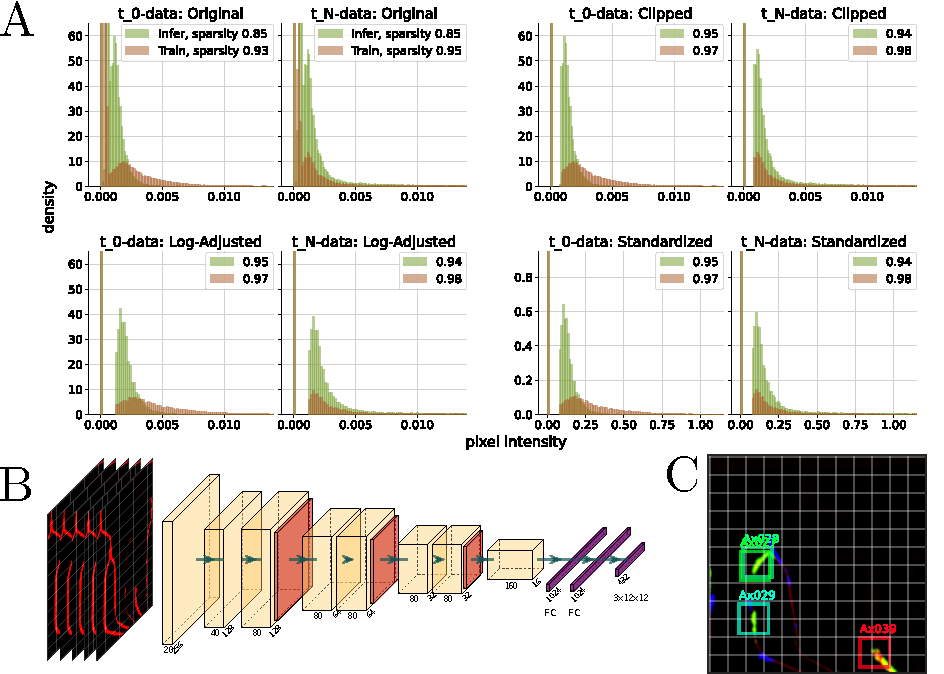
\includegraphics{M_preprocessing.pdf}
    \caption[Growth cone tracking model overview]{Growth cone tracking model
             overview. \textbf{A} CNN architecture. Each yellow block in
             represents a sequence of 2D-convolution, batch normalization
             \parencite{BN}, and Leaky ReLU \parencite{leakyrelu}. Orange layers
             stand for maximum pooling operations. FC stands for fully connected
             layers. \textbf{B} Example tile illustrating the YOLO label format.
             Each grid box can be predicted to contain a growth cone. In this
             example, 4 of 12 x 12 grid boxes are positive. Green colors in the
             tile represent positive motion (pixel intensity increased from
             frame $\rm t_0$ to $\rm t_1$), blue represents negative motion.
             Grid box size = 26 $\rm \upmu m$. \textbf{C} Minimum cost flow
             optimization illustration adopted from \parencite{MCF}. Frames are
             illustrated in gray and white background, detections within a frame
             are represented by a pre- ($o_i$), and post ($h_i$) node. Blue
             edges on the left represent costs between detections in adjacent
             frames. Coloured edges on the right indicate identity assocications
             after solving the graph. 
             } 
    \label{M_preprocessing}
\end{figure}

\paragraph{Tiling}
Each yellow block in Figure \ref{M_preprocessing} A represents a sequence of
2D-convolution, batch normalization \parencite{BN}, and Leaky ReLU
\parencite{leakyrelu}. Orange layers stand for maximum pooling operations. As
performing detection on the original resolution of 3868 x 1972 was
computationally intractable, the timelapse frames were split into 512 x 512
tiles (see Figure \ref{M_preprocessing} B and grid in Suppl. Figure
\ref{SF_training_data}). The CNN computes a convolutional feature map of 16 x 16
x 160, thus a single \textit{feature pixel} represents a region of $\rm
\frac{512}{16}$ = 32 pixels in the original 512 x 512 input image. The CNN
output resolution was a relevant consideration for its architecture, as the
detection objects of interest are small and potentially locally clustered (using
microscopy settings described in \ref{imagingsettings}, growth cones are between
4-26 pixels). If the same CNN feature output resolution was to be achieved using
original timelapse frames, the CNN output would be of shape of $\rm
\frac{3868}{32}$ x $\frac{1972}{32}$ x $160 \approx 120$ x $61$ x 160. Storing
the weights between this high-resolution CNN feature map and the first fully
connected layer exceeded  
GPU memory. An additional computational benefit is achieved by skipping empty
tiles. From visual inspection, the discontinuities between tiles did not seem to
result in decreased detection performance for growth cones near the tile edges. 

\paragraph{Detection output format}
Following the general YOLO label format, the network is trained to find a
mapping from a single tile CNN feature map to a 12 x 12 x 3 array. Here, the
first two dimensions represent a grid of the input tile, the last dimension
refers to the confidence of the respective grid box containing a growth cone,
and X-, Y grid box coordinates referring to the relative location of a growth
cone within the box (Figure \ref{M_preprocessing} B). This representation
results in the limitation, that only one growth cone can be detected per grid
box. As the example in Figure \ref{M_preprocessing} B shows, close growth cones
may still be detected as two separate identities if their centers are located in
different grid boxes. In the worst case scenario, the spatial detection
resolution of multiple growth cones is limited by the grid box size which is
equal to $\frac{512}{12} = 43$  pixels or 26 $\rm \upmu m$. This resolution was
sufficient for the application of our model as densely grouped growth cones were
the exception. \\
To drop overlapping detections, non max suppression was applied to the final
detection output according to \parencite{nms} using a minimum euclidean distance
of 23 pixels.

\paragraph{Training procedure}
The training data was split into 287 train frames (0.87), and 40 (0.13)
consecutive test frames which spanned two different PDMS micro structures. The
final model used for inference was trained on the entire dataset. Using
translation, rotation, horizontal and vertical flipping as data augmentation,
the model was trained up to convergence for 1000 epochs (Figure
\ref{R_modelresults} A). The loss function below (\ref{lossfunction}) is a
slight modification from the original.

\begin{equation}
    \lambda_{anchor}\sum_{i=0}^{S^2}\sum_{j=0}^B \mathbb{I}_{ij}^{obj}[(x_i-\hat{x}_i)^2 + (y_i-\hat{y}_i)^2 ] \\
    + \lambda_{obj}\sum_{i=0}^{S^2}\sum_{j=0}^B \mathbb{I}_{ij}^{obj}(c_i - \hat{c}_i)^2 \\
    + \lambda_{noobj}\sum_{i=0}^{S^2}\sum_{j=0}^B \mathbb{I}_{ij}^{noobj}(c_i - \hat{c}_i)^2 \\
    \label{lossfunction}
\end{equation}

\vspace{3mm}
\noindent
where $S = 12$ is the number of tiles, $B = 1$ is the number of detections per
grid box, $\mathbb{I}_{ij}^{obj}$ equals to 1 if a growth cone exists, 0
otherwise, $\mathbb{I}_{ij}^{noobj}$ equals to 0 if a growth cone exists, 1
otherwise, $c_i$ refers to the confidence that an object exists in the grid box,
and $x_i, y_i$ represent the grid box coordinates. $\hat{.}$ stands for the
ground truth label. The loss terms for predicting coordinates, object presence,
and object absence are weighted according to $\lambda_{anchor} = 45$,
$\lambda_{obj} = 54.25$, and $\lambda_{noobj} = 0.75$ respectively. The
balancing of those terms is based on the proportion of positive grid boxes which
is $\approx 0.7\%$. The initial learning rate was set to 0.0005 and decayed
with the rate $\gamma$ given in formula \ref{lrdecay}.

\begin{equation}
    \gamma = e^{-\frac{1}{10}\sqrt{x}}
    \label{lrdecay}
\end{equation}

\noindent
where $\gamma$ is multiplied with the original learning rate, and x refers to
the current epoch. \verb|Pytorch|'s Adam optimizer \parencite{adam} was used
for fitting the model with $\beta_1 = 0.9$, $\beta_2 = 0.999$.

\paragraph{Data association}
\label{data_association}
The implemented growth cone tracking model follows a classical object tracking
paradigm of splitting the problem into object detection and identity
association. For this second step, the detections produced by the YOLO-like
architecture need to be classified into unique growth cone identities that live
over several video frames. In this work, identity assignment is framed as a
graph problem where we seek minimum cost flow solutions \parencite{MCF}. At a
high level, nodes represent detections at particular frames, and edges represent
identity associations between them (see illustration in Figure
\ref{M_preprocessing} C). Each detection confidence is also represented as an
edge, which elegantly incorporates the detection model uncertainty into forming
identity trajectories through the graph and avoids the setting of explicit
detection confidence thresholds. At the basis of associating detections between
frames is the cost we assign between them. This cost can be interpreted as the
likelihood the two detections correspond to the same growth cone identity. In
contrast to other domains where visual similarity is highly relevant, because of
the large morphological variance, the edge costs here are completely based on
the spatial distance between detections. Specifically, the A* distances
\parencite{astar} between detections computed on the segmented PDMS micro
channel mask using a custom \verb|C++| implementation. This cost considers the
constraint, that growth cones can only translocate within the micro channels and
are limited in outgrowth speed. Solving the graph optimization problem includes
the constraint, that a node can only receive and emit a single edge, or in other
words, a node can only represent a single identity. As shown by \cite{MCF}, the
graph can be solved optimally and efficiently using integer linear programming.
The implementation here is based on the open-source package \verb|libmot|, using
the build-in \verb|MinCostFlowTracker|. The optimal hyperparameters listed and
explained in table \ref{MCF_params} were identified with a grid-search algorithm
on test data (see Figure \ref{R_modelresults} D). 

\begin{table*}[h]
    \begin{adjustbox}{max width=\textwidth,center}
        \begin{tabular}{@{}rrrrr@{}}
            \toprule
            Edge cost threshold      & Entry-exit cost           & Miss rate            &  &  \\
            0.7                      & 2                         & 0.6                  &  &  \vspace{5mm} \\
            \toprule
            Maximum number of misses & Minimum network flow      & Maximum network flow &  &  \\ 
            1                        & 5                         & 450                  &  &  \vspace{5mm} \\
            \toprule
            Visual similarity weight & Confidence capping method &                      &  &  \\
            0                        & \textit{scale}            &                      &  & \\
        \end{tabular}
    \end{adjustbox}
\caption[Minimum cost flow hyperparameters]
    {Minimum cost flow hyperparameters. The edge cost threshold determines if an
    edge is pruned or kept, the entry-exit cost defines the cost of creating and
    terminating identities, the maximum number of misses indicates for how many
    frames an identity can be not detected, but still not terminated, the miss
    rate determines how much cost is incurred from missing detections (low means
    high cost), minimum and maximum network flow gives the minimum and maximum
    number of identities over all frames, visual similarity weight determines
    the degree to which visual similarity between detections contributes to the
    cost, and finally the confidence capping method sets the behavior for
    confidence values above 1, where \textit{scale} means normalize to maximum
    confidence.}
\label{MCF_params}
\end{table*}

\subsubsection{Directionality inference from tracking}
\label{inferring_directionality}
Using the growth cone trajectories that lived at least for 5 timepoints, the
degree of directional growth through the PDMS micro structures can be inferred.
Analogous to the identity association cost employed for formulating the graph,
directionality inference also relies on computing A* paths on the micro channel
segmentation mask. For each detection that composes the growth cone trajectory,
we compute the shortest distance to a human-labelled target point located in the
output channel (see Suppl. Figure \ref{SF_intial_tl_preprocessing} C). Our PDMS
designs have the property, that the shortest path towards this point is
precisely the desired growth path. More intuitively, the desired growth path
towards the output channel has no detours. Thus, we can employ the A*-shortest
path towards the output channel as a proxy for confirming the correct growth
direction through the micro channels. Concretely, a correctly growing axon
should exhibit constantly decreasing A* distances towards the output channel.
Conversely, any increase in distance indicates growth in the undesired
direction. \\

A variety of metrics were considered for evaluating the degree of directional
growth through PDMS micro structures. $\Delta$ distance-to-output channel of
each axon provides a large sample size, but axon track length is not the most
direct metric of interest. To circumvent the bias of long axon tracks, we count
the number of correctly,- and incorrectly growing axons, as the basic property
of grwoth direction is more relevant then the overall covered distance. However,
since this counting overvalues slow forward growth with little convergance to
the final target location, we also analyse the number of axons reaching a
neighbour, and the output channel, respectively. Preferably, we would rely soley
on this metric, however, with the limited timelapse duration of around 5 days,
many structures exhibit a very low number of axons reaching target and
neighbours which reduces the sample size significantly. For this reason, this
metric was only employed for qualitative measures. To obtain a final metric
incorporating both forward convergence and backwards avoidance, we compute the
smoothed directionality ratio $\delta $ of the two axon counts (Equation
\ref{folddiff}).

\begin{equation}
    \delta = \frac{n_{target}+1}{n_{neighbor}+1}
    \label{folddiff}
\end{equation}
\vspace{3mm}

where $n_{target}$ and $n_{neighbor}$ refer to the number of axons reaching the
output channel and a neighbour, respectively. One is added to both quantaties to
first, avoid discarding samples with no cross-growth, and second to lower the
weights of small axon numbers. Intuitively speaking, the addition becomes
neglegiable for large values, while reducing fold-differences of small, and thus
potentially more uncertain counts. Alternative methods, for example normalizing
to the sum of the two counts elicted less distinct differences between groups.

% \subsubsection{Statistics}
% All tests reslied on non-parametric methods

\subsubsection{Analysis of axon guidance primitves}
Data for this experiment included 16-28 biological replicatess split in two
experiments, one of which was imaged at DIV 7 and 14, the other only at DIV 14.
The investigation of axon guiding design primitives relied on specifc PDMS micro
structure designs each aimed at answering a specifc qestion. In most cases,
these designs incorproated a source seeding node from which RGC axons extended
to a growth decision point. Different features were implemented in the designs
to bias the gorwth towards a specific channel. Since the segmentation of single
axons within each channel was out of scope for this work, the median
fluorescence intensity within the micro channels prior and post the decicion
point was emplyed to estimate the number of present axons. To compute the growth
bias at a disicion point, the ratio of median intensities was computed according
to equation \ref{bias_eq}. Since high pixel intensities likely translate into
more axons, we duplicated the computed bias metric $\beta$ at a particular motif
according to the pixel intensity in the inlet micro channel. This weighting of
more filled channels described in formula \ref{replic_set_eq} and
\ref{n_replic_eq} resulted in less outliers.

\begin{equation}
    \beta = \frac{I_{bias}-I_{unbias}}{I_{bias}+I_{unbias}}
    \label{bias_eq}
\end{equation}

\begin{equation}
    S = \{\beta, \dots, \beta\}
    \label{replic_set_eq}
\end{equation}

\begin{equation}
    |S| = n_{duplicates} =  \begin{cases}
        \Big \lfloor \frac{I_{inlet}-\theta} {\alpha} \Big \rfloor +1   \quad \textrm{if}  \quad I_{inlet} < 6\alpha - \theta \\\\
        6  \quad\textrm{otw.}
    \label{n_replic_eq}
    \end{cases}
\end{equation}

with $I_{bias}$, $I_{unbias}$, and $I_{inlet}$  describing the median pixel
intensity in appriximately 50 $\upmu$m of the biased channel, the unbiased
channel and the inlet channel, respectively. $S$ refers to the set of duplicated
bias measurements $\beta$ whose cardinality is defined by the input intensity
described in formula \ref{n_replic_eq}. The duplication depends on the minimum
threshold intensity $\theta$ = 0.04, and the step intensity $\alpha$ = 0.06. A
visualization clarifying the analysis methodology is shown in Suppl. Figure
\ref{SF_methods_expl} C, D and in the results, Figure \ref{R_primitives}. \\


% At the basis, metrics rely on
% the distance towards the output channel as explained above. An example of these
% distances in a particular timelapse is shown in ??.  We considered comparing the
% number of axons with negative,- and positive average slopes, as this would
% indicate the number of  correctly,- versus incorrectly growing axons,
% respectively. \\

% We need to consider the biases of each metric. Given that structures join at
% different locations, you get an inerent advantage for those that join late. \\


% growth speed is lower in more complicated designs, benefit from the mtric above \\


% metric that combines reached target, reached neighbour and directionality? 
% Correct dir 1 point, reached goal 5? Arbitrary weighting.... \\

% median vs mean gives very different story. argue for mean as outliers matter \\

% v5 has reached neighbour, reached target, v6 has directions data \\

% Speed and stagnation results 

% We chose metric...
% \clearpage

\section{Results}
\subsection{Tracking performance}
The presented model splits the tracking problem into growth cone detection and
identity association. A representative example of detections is shown in Figure
\ref{R_modelresults} B. Given the temporal stack of five image tiles, the
detection model accurately identifies growth cones in PDMS micro structure
timelapse frames. False positive detections made by the model are often
ambiguous image regions that may be interpreted as positives under less
conservative ground truth labelling. On the test set, the detector reaches a
precision of 0.73, and recall of 0.79. F1 score at a confidence threshold of
0.79 is 0.76 (Figure \ref{R_modelresults} C). A both deeper and wider CNN
architecture did show decreased performance. The ensuing step of identity
association was performed in a graph framework optimizing for minimum cost flow
solutions. Matching detection performance in tracking is challenging as in
addition to detection, identity switches, object occlusions, and suitable
identity creation-, and termination need to be considered. Using the multiple
object tracking benchmarks proposed in \cite{mot_benchmark_2015}, our tracker
achieves identity precision, recall and F1 score of 0.73, 0.68, 0.71,
respectively, which is a reasonably small drop from detection performance
(Figure \ref{R_modelresults} D). The commonly used MOTA (multiple object
tracking accuracy) metric which considers the number of false positives, false
negatives (including identity), and identity switches normalized to the number
of ground truth labels was 0.61. A more intuitive measure of tracking
performance is visualized by the top bar in Figure \ref{R_modelresults} D,
indicating the proportion of growth cones mostly tracked (0.57), partially
tracked (0.23), and mostly lost (0.2). 

Although not utilized for our application of the tracking model, axons can be
reconstructed from the growth cone track, assuming that outgrowth followed the
shortest path between detections. A visualization of the reconstructions is
shown in Suppl. Figure \ref{SF_methods_expl} B.

\begin{figure}[h!]
    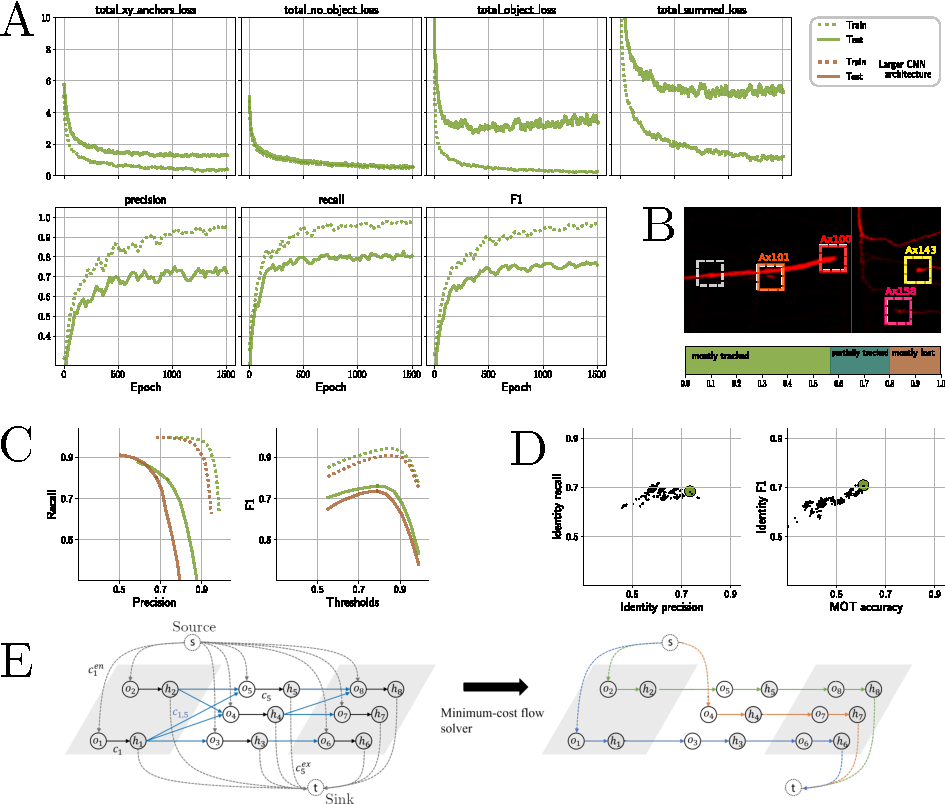
\includegraphics{R_modelresults.pdf}
    \caption[Growth cone tracking model performance]
        {Growth cone tracking model performance. \textbf{A} Loss and performance
        over 1500 training epochs. Dotted line refers to train set, solid line
        to test. The plotted loss was smoothed with an exponentially decaying
        kernel over 25 epochs, precision, recall, and F1 over 60 epochs.
        \textbf{B} Representative growth cone detection example. Dashed boxes
        are predicted, colored ones are ground truth. Scale bar = 90 $\rm \upmu
        m$. \textbf{C} Detection performance. The maximum F1 score for varying
        confidence thresholds on test set is indicated by the dot. The brown
        line shows performance for a model with wider and deeper architecture.
        Legend in A applies. \textbf{D} Model growth cone tracking performance.
        Identity precision and recall incorporate classification of correct
        identity. Each black dot represents the performance using one set of
        hyperparameters, the green dot represents the highest scoring set (see
        Table \ref{MCF_params}) where identity F1 was 0.71, MOT accuracy 0.61.
        MOT accuracy measures the number of false positives, false negatives,
        and identity switches normalized to the number of ground truth labels.
        The top bar visualizes the proportion of growth cones that were mostly
        tracked (green, $>$80\% identity lifetime tracked), mostly lost (brown,
        $<$20\%), and partially tracked (dark green, between 20-80\%).
        } 
    \label{R_modelresults}
\end{figure}

\subsection{Micro structure designs}
The tracking model described above was used for evaluating a set of 21 PDMS
micro structures designed for directing axon growth from multiple source regions
towards a common target. These designs are the result of unpublished previous
work extensively described in Supplementary Information 1. In short, the 21
designs test a set of presumably relevant variables that yield directional
axonal growth, including different types of 2-joints, joint placements and joint
frequencies. Figure \ref{R_designs} illustrates the specific features
implemented in the different designs. Design 05 on the right exemplifies the
general PDMS architecture composed of four source wells, the final lane,
the higher output channel with added diffusion wells and finally a target
stomach \parencite{forro}. 

\begin{figure}[h!]
    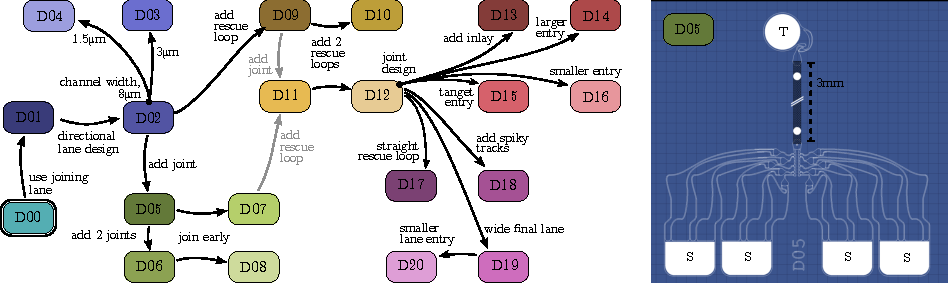
\includegraphics{R_designs.pdf}
    \caption[PDMS micro structure designs]
        {PDMS micro structure designs. The left illustration provides an
        overview of the 20 modelled micro structures including their
        distinguishing design features. Starting from Design 00 (D00), the arrows
        can be interpreted as an implemented design change. For example, D05 and
        D06 differ specifically in the number of 2-joints. For more details on
        the single designs see Suppl. Information 1. On the right, the D05 design is
        shown as an example. Filled white regions are openings, white lines
        indicate 6 $\upmu$m high channels, the black region represents the 75
        $\upmu$m high output channel (note discontinuity for illustrative
        reason). RGC spheroids are seeded in the source wells (S), the thalamic
        attractor is placed in the target well (T). Grid dimension 100 $\upmu$m.
        The magnification highlights the two main merging structures, 2-joints
        and final lane joints.} 
    \label{R_designs}
\end{figure}


\subsection{Between dataset variance}
The translocation of RGC growth cones was tracked over a period of five days to
infer the degree of directional growth through new PDMS micro structure designs.
The directionality was evaluated based on the A* distance-to-output channel over
time (see Methods \ref{inferring_directionality}). Figure \ref{R_more_metrics} A
shows this inference of directionality from output channel distances for
tracking axons in Design 05. Axons that grow towards the output channel exhibit
smaller distances over time, thus the $\Delta$ distance towards the output
channel is negative for directionally growing axons. These distances form the 
basis of subsequent analysis steps.\\

Tracking was performed on two datasets obtained from experiments with sightly
differing setups. While Dataset4 was acquired using thalamus spheroids placed in
stomachs (see Figure \ref{R_designs} right), Dataset3 used free floating
thalamic tissue pieces enclosed by PDMS frames to locally increase attractor
concentration. Dataset3 and 4 exhibit a collection of significant differences.
Figure \ref{R_more_metrics} B highlights the variation of growth directionality
between the two. During the initial outgrowth phase, $\Delta$ distances
collectively decrease for all designs by 300 $\upmu$m in both datasets. Albeit
with increasing variance, this average distance is kept throughout, indicating a
dominance of non-moving growth cones. While the averages are comparable, the
variance of directionality differs vastly between Dataset3 and 4. In contrast to
Dataset3, Dataset4 shows only marginal differences between designs, and the
overall variance is smaller. This discrepancy is condensed in Figure
\ref{R_more_metrics} B (right) with the temporal dimension collapsed. To better
identify differences in directionality between designs, subsequent analysis was
conducted on the interval with maximum variance, DIV 3.5 to 6 (see dashed line).

\begin{figure}[h!]
    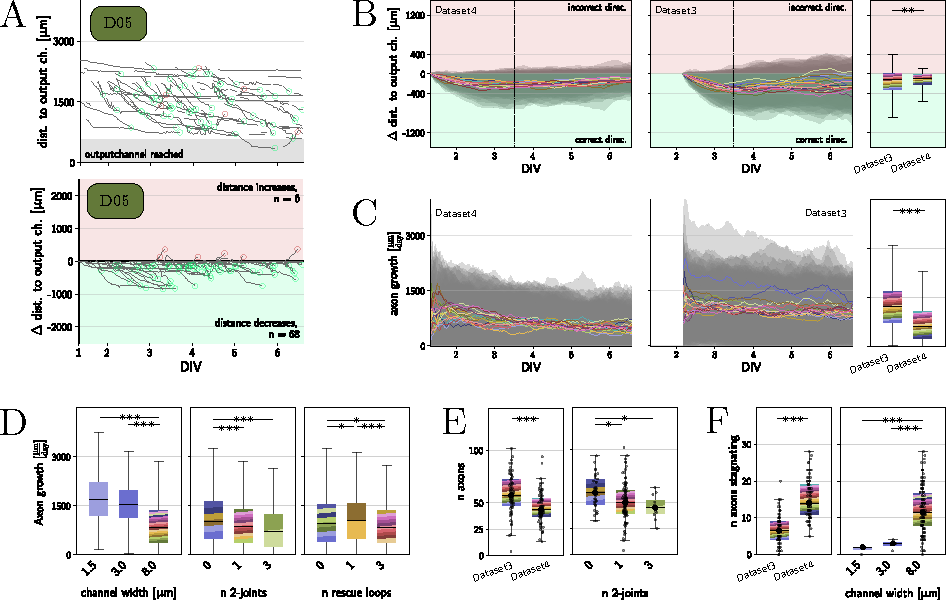
\includegraphics{R_more_metrics.pdf}
    \caption[Between dataset variance and axonal viability]
        {Between dataset variance and axonal viability. \textbf{A} Inferring
        directionality from distance-to-output channel exemplified in design 5.
        Each of the gray lines represents an axon identity, axons in the light
        gray region are inside the output channel. Subtracting the initial
        distance to the output channel yields the bottom plot. Green or red
        circles mark axons that grew at least 50 $\upmu$m in the correct or
        incorrect direction, respectively. Count is given in corners. \textbf{B}
        Median growth directionality over time. Axon wise $\Delta$
        directionality is computed by subtracting first- from last
        distance-to-output channel. Each colored line represents a design
        following the color code in Figure \ref{R_designs}, gray regions
        indicate the standard deviation. \textbf{C} Axon growth velocity over
        time. \textbf{D} Axon growth velocity split by design feature. As for
        all following boxplots, whiskers represent 1.5 x inter quartile range
        (IQR), and colors represent the 21 designs composing the distribution
        according to the color code in Figure \ref{R_designs}. \textbf{E} Number
        of axons identified in one half of a PDMS micro structure. Single dots
        represent datapoints composing the distribution. \textbf{E} Number of
        stagnating axons identified in one half of a PDMS micro structure.
        Kruskal-Wallis test was used for non-parametric group comparisons,
        subsequently, the single comparisons were made using Mann-Whitney-U test
        with Holm-Bonferroni correction. * indicates p$<$0.05, ** p$<$0.005, and
        *** p$<$0.0005. Applies for subsequent figures.} 
    \label{R_more_metrics}
\end{figure}



\subsection{Axonal viability across datasets \& designs}
PDMS micro structure designs primarily focus on achieving directional growth
towards the output channel. While this metric is crucial, as with any metric,
ignoring other relevant factors may result in poor overall performance. In our
case, these other relevant factors are indicators of neural viability, including
axonal outgrowth velocity, frequency of outgrowth, long-term survival and
electrical transmission efficacy. While screening all these factors along
side directionality performance was out of scope for this work, the tracking of
growth cones yielded insights into frequency and velocity of axonal outgrowth.
Intuitively, the frequency of outgrowth is directly derived from the number of
unique axon identities. The growth velocity in
[$\frac{\mathrm{\upmu}\mathrm{m}}{\mathrm{day}}$] was determined from the slope
of distance-to-output channel over time (Figure \ref{R_more_metrics} A). This
allowed for a further metric, namely the classification of stagnating axons.
Here, we defined axons as stagnating if the standard deviation of growth
velocity over the last 5 h of detection was below 12
[$\frac{\mathrm{\upmu}\mathrm{m}}{\mathrm{day}}$]. In Figure
\ref{R_more_metrics} A (top) stagnating axons clearly appear as horizontal
lines. \\

In accordance with the directionality discrepancy between datasets described
above, the complementary metrics of outgrowth frequency, outgrowth velocity and
stagnation frequency differ significantly between datasets (Figure
\ref{R_more_metrics} C,E,F). Figure \ref{R_more_metrics} C illustrates the
growth speed over time for both datasets. Initially, the growth velocity is
approximately 1100 [$\frac{\mathrm{\upmu}\mathrm{m}}{\mathrm{day}}$] with high
variance. While the average growth velocity and variance decline over time in
Dataset4, Dataset3 maintains the high initial outgrowth velocity. As expected,
the number of stagnating axons per PDMS micro structure is significantly higher
in Dataset4 (Figure \ref{R_more_metrics} F). Lastly, the outgrowth frequency is
significantly lower in Dataset4 (Figure \ref{R_more_metrics} E). \\

So far, the data was only grouped by dataset. To reveal potential effects of
different PDMS designs on the axonal viability metrics, the dataset may be split
by design features, such as the channel width, the number of rescue loops, and
the number of 2-joints. Figure \ref{R_more_metrics} D shows the effect of these
three features on axonal growth velocity. Especially the PDMS micro channel
width has a highly significant effect. By almost completely eliminating
stagnation (Figure \ref{R_more_metrics} F),  the Designs 03 and 04 which
implement 3 and 1.5 $\upmu$m wide channels respectively exhibit approximately
double the growth velocity compared to 8 $\upmu$m designs (see
\verb|D04_tracking.mp4|). A smaller yet highly significant relationship was
identified between the number of 2-joints and rescue loops. Omitting both of
these elements yields significantly higher growth velocity. While the number of
2-joints seems qualitatively anti correlated with growth velocity (0 $>$ 1 $>$
3), the number of rescue loops is not, as designs with one rescue loop show
significantly faster growth compared to designs with zero loops. Similar to
growth velocity, the number of 2-joints seems to have a small negative effect on
axonal outgrowth frequency (Figure \ref{R_more_metrics} E).

\begin{figure}[h!]
    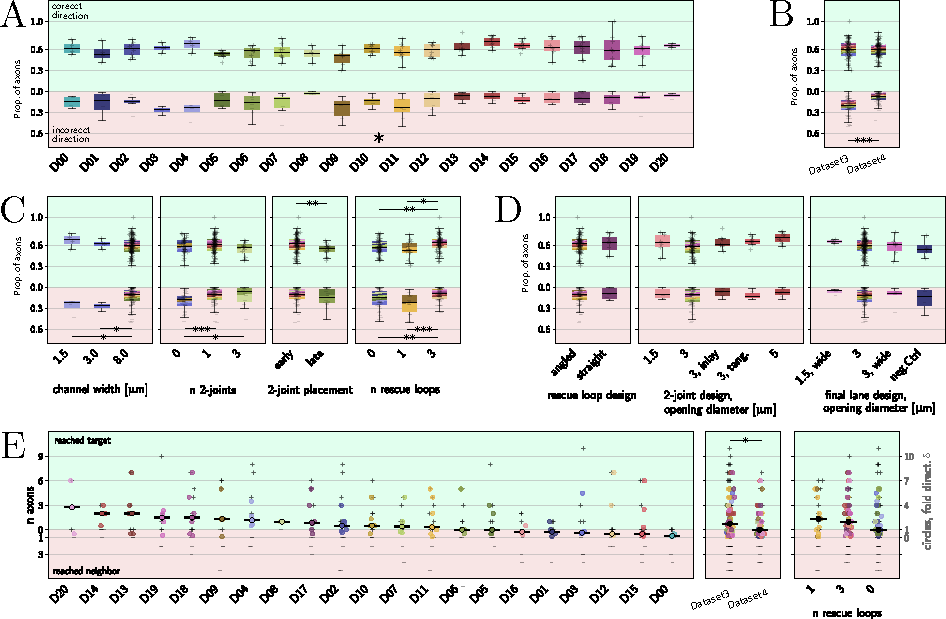
\includegraphics{R_directionality.pdf}
    \caption[Directionality in PDMS designs]
        {Directionality in PDMS designs. \textbf{A} Proportion of correctly,-
        and incorrectly growing axons in one half of a PDMS micro structure.
        Axons were counted if the $\Delta$ distance was above 50 $\upmu$m. Faint
        + and - symbols compose the distributions, respectively. Applies for B,
        C and D as well. Star indicates that Kruskal-Wallis test evaluates the
        design as a significant factor for backwards growth, but single
        comparisons don't pass Mann-Whitney-U test with Holm-Bonferroni
        correction. \textbf{B} Number of correctly,- and incorrectly growing
        axons split by dataset. \textbf{C} Number of correctly,- and incorrectly
        growing axons split by significant features. \textbf{D} Number of
        correctly,- and incorrectly growing axons split by non-significant
        features. One other non-significant feature, the use of spiky tracts, is
        shown in Suppl. Figure \ref{SF_methods_expl} E. \textbf{E} PDMS micro
        structure designs ranked by $\updelta$ fold directionality.
        Corresponding to the left y-axis labels, + and - symbols represent the
        number of axons that reached the output channel or neighbor,
        $n_{target}$, $n_{neighbour}$, respectively. The colored circles
        represent the smoothed $\updelta$ fold directionality computed from
        these two counts as formulated in equation \ref{folddiff}, medians are
        indicated by horizontal lines. The axis labelling on the right applies
        for all circles. } 
    \label{R_directionality}
\end{figure}

\subsection{Directionality in PDMS designs}
Tracking growth cones provides insights into interesting axonal growth
properties and their dependence on design features. However, the primary
intention of tracking was to identify PDMS micro structure designs that result
in high directional growth from seeding wells to output channel. As shown in
Figure \ref{R_more_metrics} A, the directionality is evaluated based on the A*
distance-to-output channel over time. A simple approach suitable for large
effect sizes is to compare distributions of axon wise $\Delta$ distances (see
Figure \ref{R_more_metrics} B, right). This method favors long axon tracks,
which is not of direct interest. Rather, the qualitative property of growing in
the correct,- or incorrect direction is relevant (see circles in Figure
\ref{R_more_metrics} A).  Figure \ref{R_directionality} A summarizes those
counts of axons for all 21 designs, normalized to the total number of observed
axons. While none of the single comparisons pass statistical significance with
Holm-Bonferroni correction, the factor \textit{design} has a significant impact
on backwards growth. Forward growth counts exceed backward growth across all
designs since the initial outgrowth is strongly biased towards forward growth.
With approximately 65 \%, the highest median of forward growing axons is
observed in  design 4 implementing 1.5 $\upmu$m wide channels. However, this
strong forward bias comes at the cost of the relatively high backward growth of
25 \%, which is also observed in design 3 using 3 $\upmu$m wide channels. In
contrast, design 8 implementing frequent, late merging shows nearly no backward
growing axons paired with average forward growth. The Designs 12-20 which share
the same general architecture but vary in specific motif designs collectively
exhibit few (around 10 \%) backwards growing axons. The forward growth
distribution of design 18 using spiky tracts on unpreferred edges has the
longest positive tail. \\

Grouping the data by design features instead of design can reveal more distinct
trends. Figure \ref{R_directionality} C and D summarize significant and
non-significant effects, respectively. As mentioned before, smaller channel
widths increase both forward,- and backward bias, however, only the backward
effect is statistically significant. Another significant design feature is the
number of 2-joints, or merging structures. Using one or three instead of none
yields significantly lower backwards growth, whilst not affecting the forward
bias. Conversely, forward bias is significantly impacted by the placement of
2-joints but does not have an effect on backwards growth counts. Joining
channels early yields a significant increase in forward growth of approximately
10 \%. Lastly, the number of rescue loops has an impact on both forward,- and
backwards growth. Implementing three instead of one or none rescue loops prior
to each 2-joint reduces the proportion of backwards growing axons. Forward bias
was significantly increased between three and fewer than three rescue loops. No
significant effects were observed for angled versus straight rescue loop
designs, spiky tracts, different variants of 2-joints and modifications to the
final lane design (Figure \ref{R_directionality} D). \\

As mentioned in the methods (\ref{inferring_directionality}), focusing solely on
growth direction counts may overestimate the performance of designs with low to
medium forward convergence that do not reach critical joining areas. This is
observed when splitting by dataset origin, as shown in Figure
\ref{R_directionality} B. Timelapse videos of Dataset4 show only few axons
reaching 2-joints or final lane, thus backwards growth is significantly biased
towards lower values. To compute an interpretable directionality metric that
mitigates this directionality overestimation, we compute the ratio of axons
reaching the output channel and axons reaching neighbors. Ranked by performance,
both single axon counts and $\delta$ fold directionality are shown in Figure
\ref{R_directionality} E. Due to many samples showing neither target,- nor
neighbor grown axons, $\updelta$ measures were limited to fewer samples,
resulting in almost no significant differences. Still, the metric provides
valuable qualitative insights in comparison to directional counts in Figure
\ref{R_directionality} A. Consistent with good performance on growth direction
counts, the five Designs 20, 14, 13, 19, and 18 show $\updelta$ fold
directionality between almost 4 and 2.5 (see \verb|D20_tracking.mp4|). Hinting
at the potential discrepancy between the two metrics, design 9 $\updelta$
performance shows a tendency to be better than what relative growth direction
counts indicate. $\updelta$ below 1 is observed in Design 00 (see
\verb|D00_tracking.mp4|), 15, 12, 03, 01, and 16. These designs implementing no
final lane, a final lane with,- and without directional promoting geometry, and
2-joints with medium-sized and tangent entries exhibit more axons reaching the
neighbor than the output channel. The only significant differences in $\updelta$
are observed when grouping by dataset. In sharp contrast to results in Figure
\ref{R_directionality} B, design measurements originating from Dataset4 show
lower performance than those from Dataset3, highlighting the overestimation bias
of counted growth direction clearly. In line with the observation in Figure
\ref{R_directionality} C, though not significant, the implementation of rescue
loops tends to have a positive effect on the $\updelta$ metric (Figure
\ref{R_directionality} E, right).

\subsection{Axon guidance design primitves}
\begin{figure}[t!]
    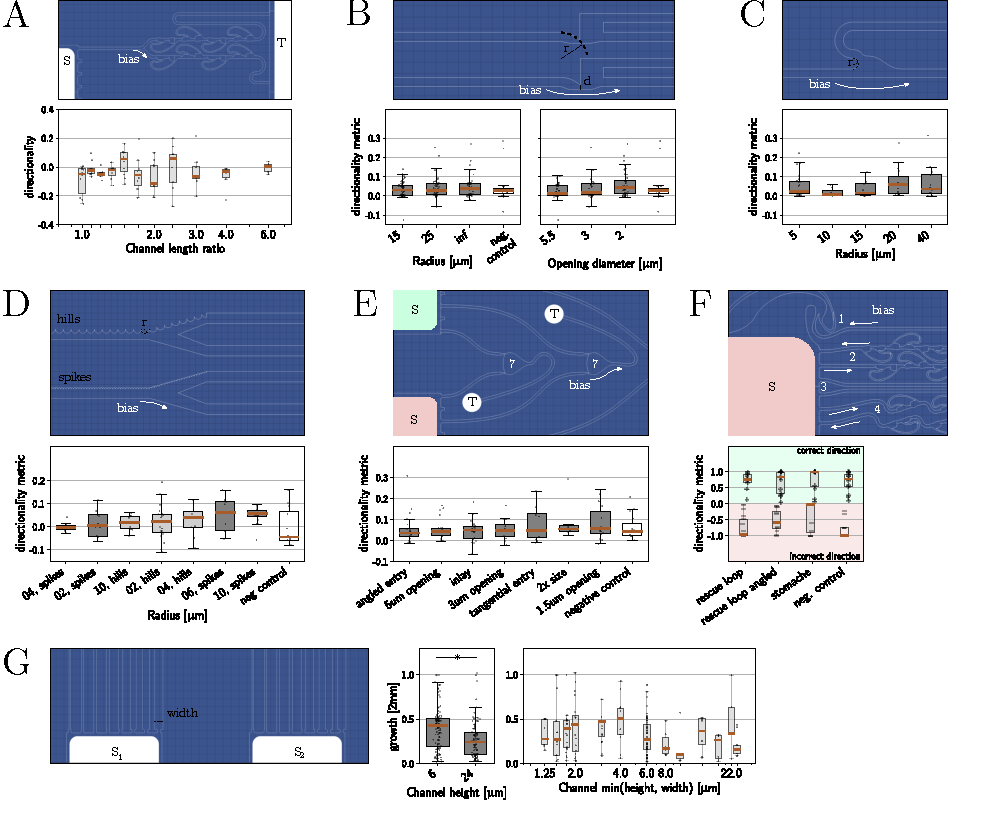
\includegraphics{R_primitives.pdf}
    \caption[Axon guidance primitives in micro structure designs]
        {Axon guidance primitives in micro structure designs. All PDMS micro
        structure designs show RGC left-to-right growth from seeding well (S) to
        target well (T). \textbf{A} Effect of cue gradient on directional growth
        introduced by varying attractor channel length from seeding well (S)
        towards the thalamic cue source (T). A ratio of 6 translates into
        channels with a length 480 $\upmu$m, and 6 x 480$\upmu$m. \textbf{B}
        Edge transition motif parameters radius r and opening diameter d. The
        negative control omits the edge transition feature. Infinite r refers to
        designs where the input channel is tilted up by 45$^{\circ}$. \textbf{C}
        Radial detachment for varying radii r. \textbf{D} Introduction of
        edge-detaching features. Light gray bars used hills, dark gray indicates
        the use of spikes instead.\textbf{E} 2-joint or merging structure
        design. Source wells (S) are seeded with GFP, and RFP labelled RGCs,
        respectively. Here, the bias metric $\beta$ replaces $I_{bias}$ with
        $I_{inlet}$ in equation \ref{bias_eq}. The shown 2-joint design is
        number 4, using an opening diameter 1.5 $\upmu$m. \textbf{F}
        Directionality constraint growth. Similar to E but here connected with
        asymmetric channels, two opposing wells are seeded with GFP,- (not
        shown) and RFP labelled RGCs. Four different design motifs are compared
        in terms of maximum distance reached. Red lines indicate median
        forward,- (green) and backward (red) distance reached. As in previous
        figures, stars without lines indicate Kruskal-Wallis test evaluating to
        p$<$0.05, lines translate into subsequent Mann-Whitney-U tests also
        outputting p$<$0.05.} 
    \label{R_primitives}
\end{figure}
By tracking axons through PDMS channels during the initial growth phase, we
identified micro structure designs with notable directionality. While number,-
and placement of 2 joints, channel width and number of rescue loops had a
significant impact on directionality performance, more settle and specific
design motif alterations introduced to the final lane and 2-joints did not
elicit significant differences. To identify PDMS motif designs that impact
directional growth, we designed PDMS micro structures that answer specific
questions about both chemical and structural axon guidance. The experimental
setups and results of testing these guidance primitives are presented in Figure
\ref{R_primitives}. \\

Chemical guidance was investigated by creating a differential attractor cue
concentration at a growth decision point (Figure \ref{R_primitives} A). The aim
was to create a chemical gradient by introducing differential channel lengths
towards a seeding well containing a thalamus spheroid. We do do not observe
biased growth along the shortest path towards an attractor, not even if the
ratio between the two channel lengths is as high as six. \\

PDMS geometry based axon guidance relies on the tendency of axons to adhere to
edges and avoid sharp turns. In scenarios such as channel merging, final lane
merging, and rescue loops, we aim to direct axon growth towards a preferred edge
that guides towards the preferred direction. Figure \ref{R_primitives} B shows
the results of comparing edge transition motifs parameterized by two factors,
the radius r guiding towards the preferred edge, and the opening diameter d
between edges. Both factors significantly bias growth direction, however, no
single comparisons pass significance with Holm-Bonferroni correction.
Qualitatively, it seems that larger radii guiding towards the preferred edge
improve edge transitions, but returns diminish for very large radii. Also,
successful edge transition seems to occur more frequently when the opening
diameter is 2 $\upmu$m instead of 5.5 or 3. Both 5.5 and 3 $\upmu$m openings
show little growth bias difference with the control, indicating the importance
of small diameters. In Figure \ref{R_directionality} C, we aimed to test axon
detachment behavior when growing along differentially sharp radii. Although
previously published stomach structures seem to rely on this principle
\parencite{forro}, we do not find a significant relationship between small radii
supposedly inducing an edge transition, and a directional growth bias. The
previous two primitives investigated the process of edge transitioning at
joining or rescuing motifs, however, one may also consider channel designs that
promote growth on preferred edges a priori. Figure \ref{R_primitives} D shows
experiments implementing hill,- and spike-like edge features of varying radius
to drive axon growth on the opposing edge. Again, while this factor passes
significance, single comparisons do not. It seems however, as if both hills and
spikes of medium radius (4, and 6 $\upmu$m) are able to bias growth in one
direction. \\

The primitives investigated in Figure \ref{R_directionality} A-D aimed to find
optimal low-level building blocks for designing axon-guiding micro structures.
In Figure \ref{R_primitives} E and F, we reduce the abstraction level in testing
practical PDMS micro structure motifs to merge channels and achieve directional
growth. 8 different 2-joint designs were tested in terms of their ability to
merge two channels with minimal cross growth (Figure \ref{R_primitives} E). Due
to the control performing surprisingly well, the only 2-joint significantly
differing from control after multiple testing correction was design 1 using
angled joint entries. The highest median growth bias was observed in 2-joints
using tangential edge transitions. Lastly, we tested the ability of three
different designs to achieve directional growth from one node to another (Figure
\ref{R_primitives} F). Although again not statistically significant, previously
published stomach structures show very low median backwards growth. Angled
rescue loops seem to perform slightly better than non-angled ones in preventing
backwards growth. Forward growth is not negatively affected in any of the
designs.


\clearpage

\section{Discussion}


\subsection{Model architecture and generalization}

treating numerical variables as categoric ones 

concern with viability results for n 2-joints: design 8 only in Dataset4, which
has generally lower growth. 
\clearpage

\section{Supplementary Figures}
\begin{suppfigure}[h!]
    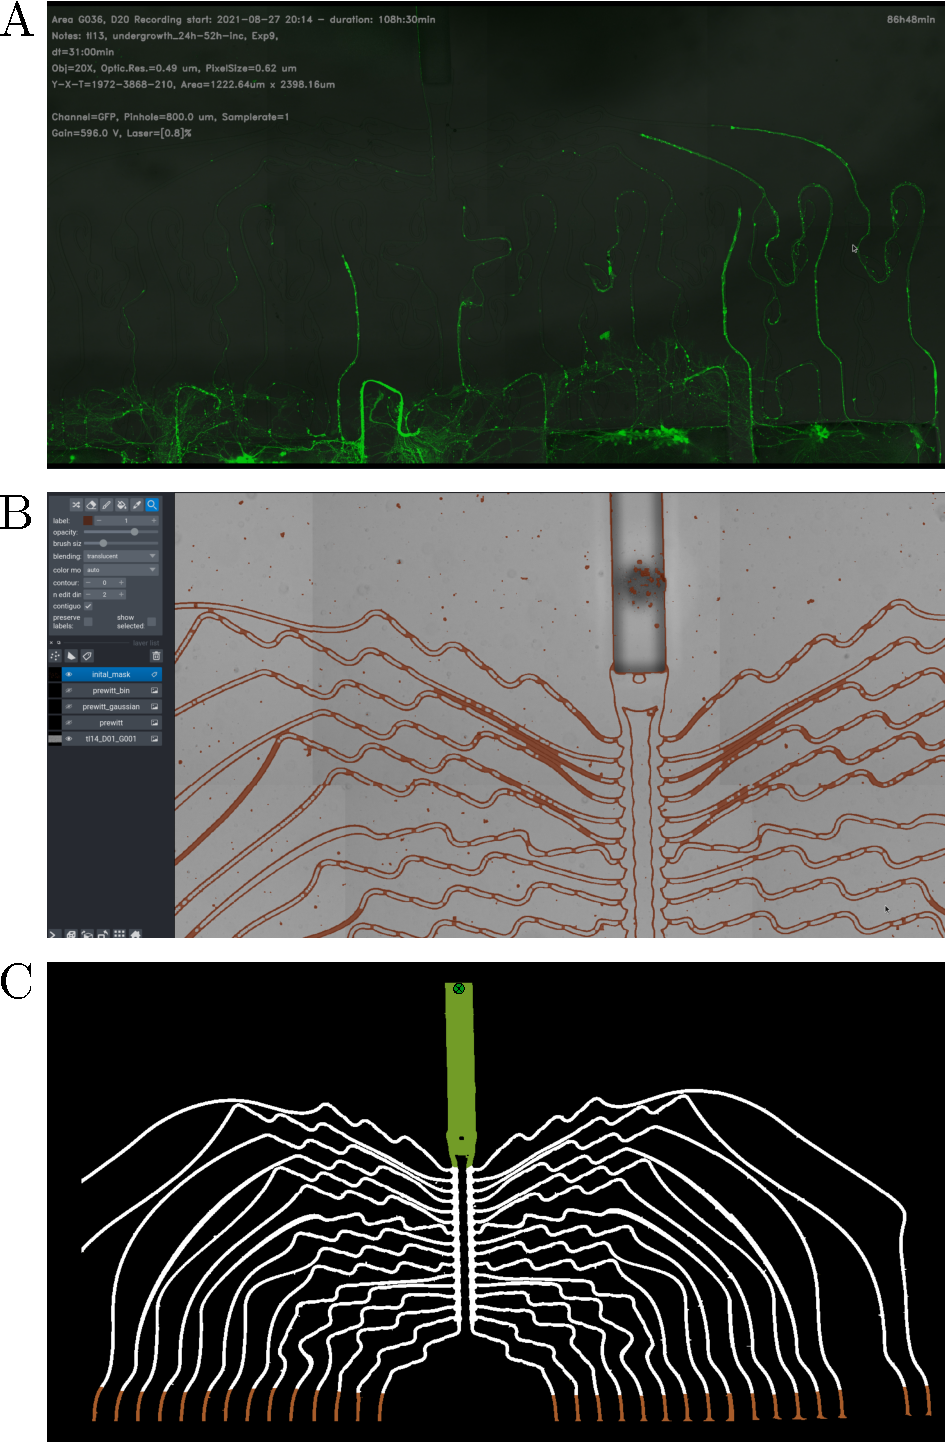
\includegraphics{SF_intial_tl_preprocessing.pdf}
    \caption[Initial timelapse preprocessing steps]{Initial timelapse
             preprocessing steps. \textbf{A} A snapshot of the exported video
             including the relevant metadata of the recording. \textbf{B} The
             napari image viewer interface with the edge segmentation layer in
             brown. \textbf{C} The manually segmented binary mask of the micro
             channels in non-black, the output channel in green, and the exiting
             channels in brown. The green dot in the output channel marks the
             target point of the PDMS design.}
    \label{SF_intial_tl_preprocessing}
\end{suppfigure}

\begin{suppfigure}[t!]
    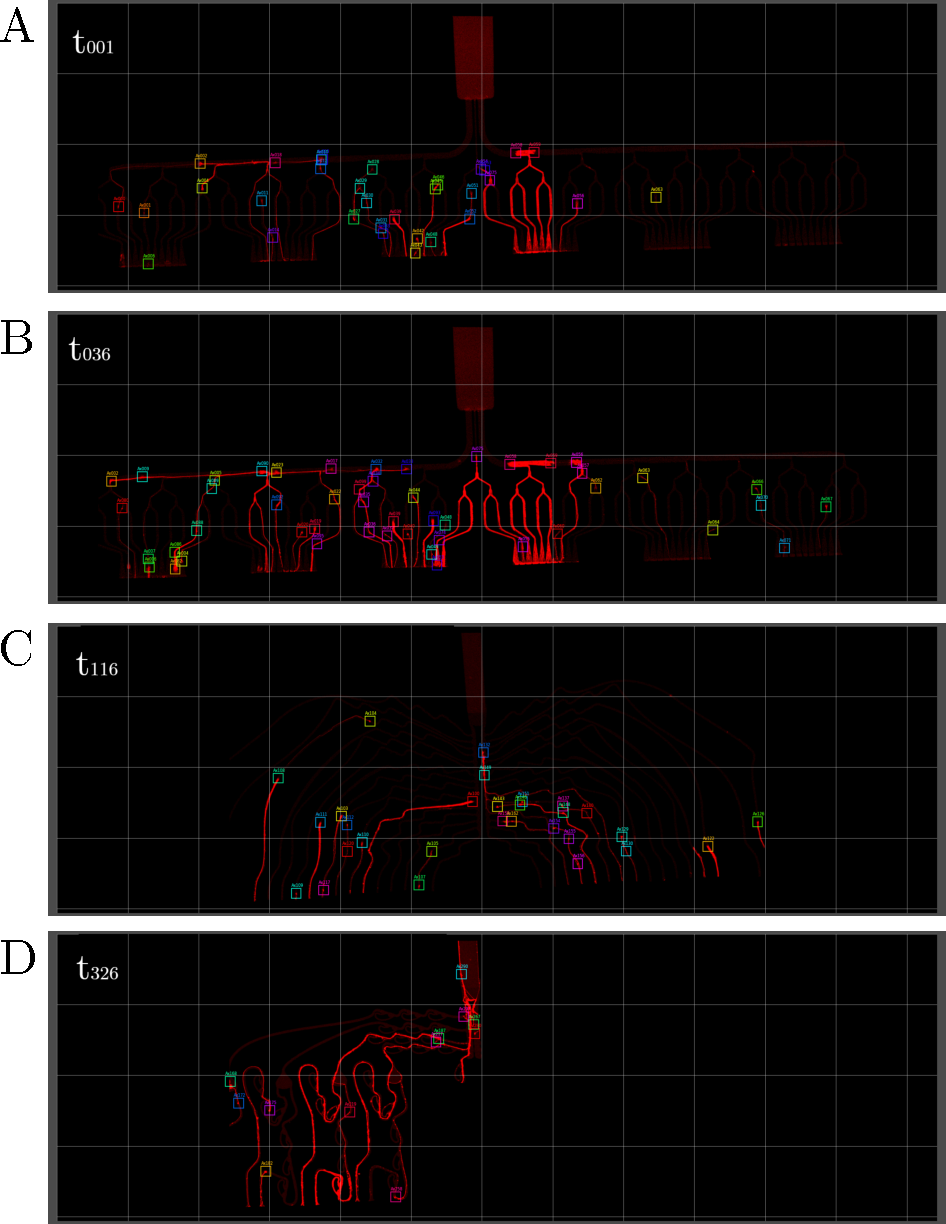
\includegraphics{SF_training_data.pdf}
    \caption[Labelled training data examples]{Labelled training data examples.
             \textbf{A} shows the first frame of the training data sequence.
             Each box represents a growth cone, the color indicates the identity
             over consecutive frames. \textbf{B} shows the last frame of
             Dataset1. \textbf{C} shows the last frame of Dataset2, PDMS micro
             structure 1 (compare Table \ref{datasets_table}). \textbf{D} shows
             the last frame of Dataset2, PDMS micro structure 2. Gridsize = 317
             $\rm\upmu m$.} 
    \label{SF_training_data}
\end{suppfigure}

\begin{suppfigure}[t!]
    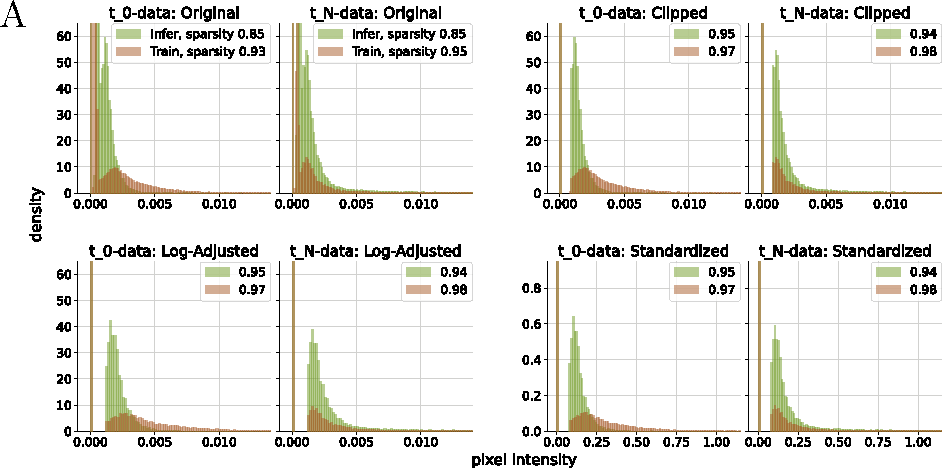
\includegraphics{SF_image_preproc.pdf}
    \caption[Preprocessing effects on pixel intensity
            distributions]{Preprocessing effects on pixel intensity
            distributions. \textbf{A} Pixel intensity distribution of training-,
            and inference data at $\rm t_0$ and $\rm t_N$ over three major
            preprocessing steps. The two plots top left show the initial pixel
            intensity distributions, top right after clipping, bottom left after
            log adjusting, and bottom right after standardization. Histograms on
            the left were obtained from sampling $10^6$ pixel values from the
            first frame, histograms on the right from the last respective frame.
            The inference data to produce the histograms (brown) was taken from
            a representative image sequence from Dataset3 (see Table
            \ref{datasets_table}). The number in the legend indicates the
            proportion of image values equal to zero (sparsity). Note that
            outlier intensity values are not shown. 
             } 
    \label{SF_image_preproc}
\end{suppfigure}

\begin{suppfigure}[t!]
    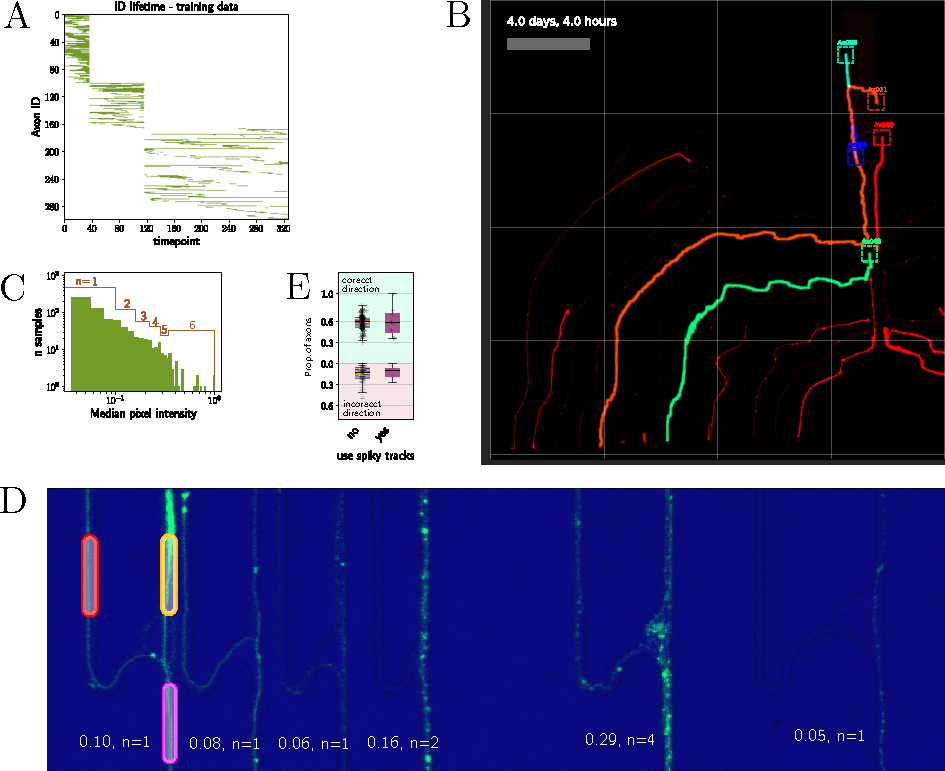
\includegraphics{SF_methods_expl.pdf}
    \caption[Methodology illustrations]{Methodology illustrations. \textbf{A}
             illustrates the axon identify lifetime. A green point on this pixel
             map indicates that a label exists for the matching axon identity
             and frame. The three clusters originate from the concatenation of
             three PDMS micro structure timelapse videos. \textbf{B} Axon
             reconstruction from growth cone track. For clarity, only a subset
             of identified axons is drawn. Gray bar width is 200 $\upmu$m.
             \textbf{C} Estimation of n axons/ duplicates (brown) from median
             intensities (green) for primitives analysis. Note double log
             scales. \textbf{D} Design primitives analysis example. Shown is the
             intermediate analysis output for the radial detachment primitive.
             The pink, yellow, and red boxes indicate the regions for computing
             inlet, biased, and unbiased median intensity, respectively.
             Annotated numbers refer to inlet median intensity and the resulting
             number of duplicates n. \textbf{E} Proportion of axons growing in
             the correct,- and incorrect direction, respectively. Split by using
             spiky tracks or not. This extends the panel from Figure
             \ref{R_directionality} D summarizing tje design features not
             significantly effecting directionality. Moved for visual clarity.}
    \label{SF_methods_expl}
    % \label{SF_labelling}
\end{suppfigure}


% \begin{suppfigure}
%     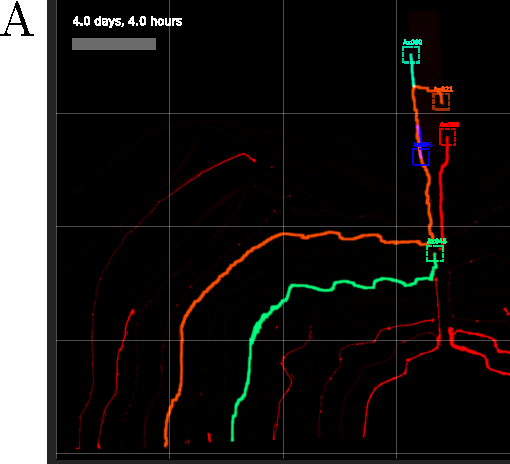
\includegraphics{SP_ax_reconstructions.pdf}
%     \caption[Axon reconstruction from growth cone track]
%     {} 
%     \label{SP_ax_reconstructions}
% \end{suppfigure}



% \begin{suppfigure}
%     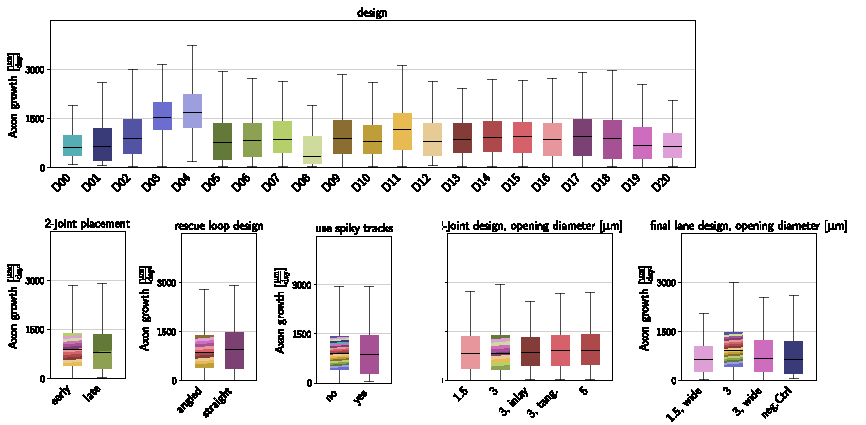
\includegraphics{SF_growthspeed.pdf}
%     \caption[Axonal growth velocity]
%     {Axonal growth velocity. Significance is not shown.} 
%     \label{SF_growthspeed}
% \end{suppfigure}


% \begin{suppfigure}
%     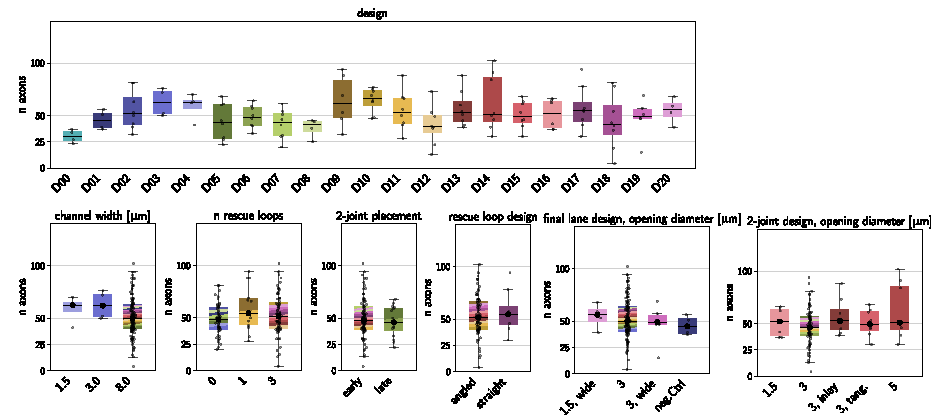
\includegraphics{SF_naxons.pdf}
%     \caption[Axon outgrowth frequency]
%     {Axon outgrowth frequency. Significance is not shown.} 
%     \label{SF_naxons}
% \end{suppfigure}


% \begin{suppfigure}
%     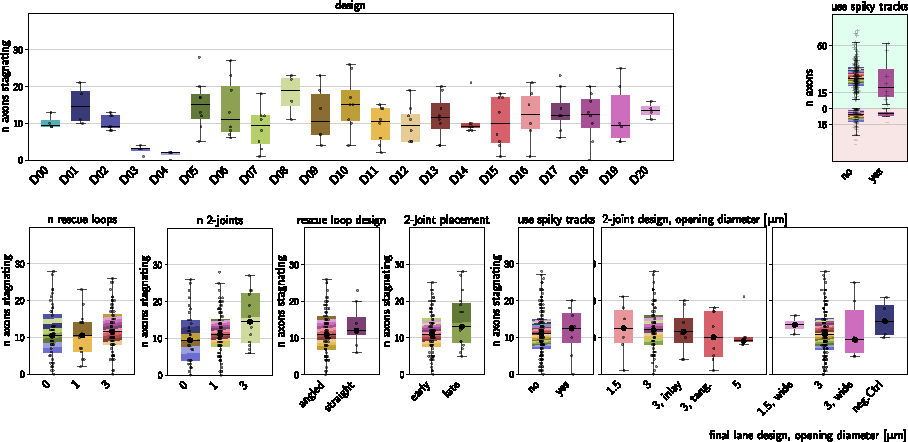
\includegraphics{SF_stagnation.pdf}
%     \caption[Number of axons stagnating]
%     {Number of axons stagnating. Significance is not shown. Top right plot shows
%     counts of axons growing incorrectly (red), and correctly (green) for a
%     feature that did not show significant effects.} 
%     \label{SF_stagnation}
% \end{suppfigure}

% \begin{suppfigure}
%     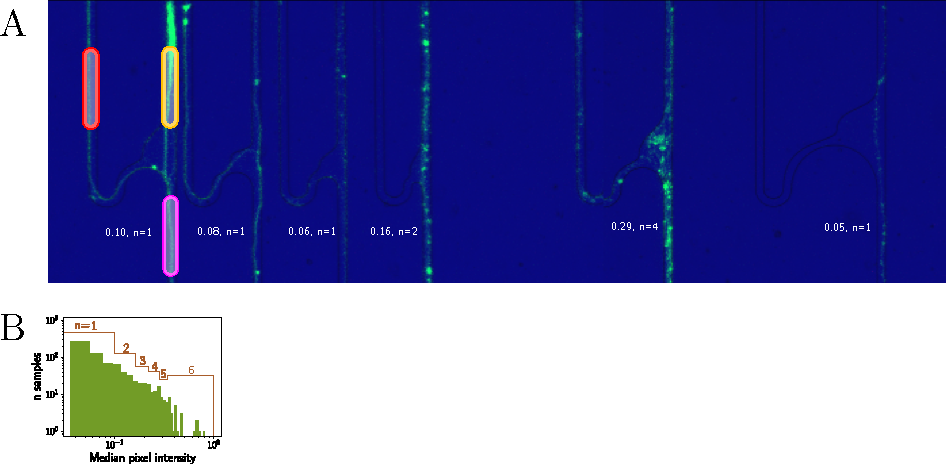
\includegraphics{SF_prim_analysis.pdf}
%     \caption[Design primitives analysis methodology]
%     {. \textbf{A} Design primitives analysis example. Shown is the intermediate
%     analysis output for the radial detachment primitive. The pink, yellow, and
%     red boxes indicate the regions for computing inlet, biased, and unbiased
%     median intensity, respectively. Annotated numbers refer to inlet median
%     intensity and the resulting number of duplicates n. } 
    
%     \label{SF_prim_analysis}
% \end{suppfigure}
\clearpage

\printbibliography

\end{document}